% oss-plantilla: oss-2026.11
% Preámbulo corporativo fijo. No editar en sd-NN.tex: exportar_latex.py verificar lo compara byte a byte.
% Para cambiar el formato, editar esta plantilla u oss.sty y subir la versión de la primera línea.
\PassOptionsToPackage{unicode}{hyperref}
\PassOptionsToPackage{hyphens}{url}
\documentclass[11pt]{article}
\usepackage{amsmath,amssymb}
\usepackage{iftex}
\ifPDFTeX
  % Prism y otros editores en la nube: pdfLaTeX con Helvetica como familia por defecto.
  \usepackage[T1]{fontenc}
  \usepackage[utf8]{inputenc}
  \usepackage{textcomp}
  \usepackage[scaled=0.92]{helvet}
  \renewcommand{\familydefault}{\sfdefault}
  \DeclareUnicodeCharacter{2264}{\ensuremath{\leq}}
  \DeclareUnicodeCharacter{2265}{\ensuremath{\geq}}
  \DeclareUnicodeCharacter{2260}{\ensuremath{\neq}}
  \DeclareUnicodeCharacter{2248}{\ensuremath{\approx}}
  \DeclareUnicodeCharacter{2190}{\ensuremath{\leftarrow}}
  \DeclareUnicodeCharacter{2192}{\ensuremath{\rightarrow}}
  \DeclareUnicodeCharacter{25CF}{\ensuremath{\bullet}}
  \DeclareUnicodeCharacter{2713}{\ensuremath{\checkmark}}
\else
  % XeLaTeX/LuaLaTeX (compilación oficial local): DejaVu Sans.
  \usepackage{fontspec}
  \defaultfontfeatures{Ligatures=TeX,Scale=MatchLowercase}
  \setmainfont{DejaVu Sans}
  \setsansfont{DejaVu Sans}
  \setmonofont{DejaVu Sans Mono}
\fi
\usepackage[letterpaper,margin=20mm]{geometry}
\usepackage{microtype}
\usepackage{parskip}
\usepackage{xcolor}
\usepackage{longtable,booktabs,array}
\usepackage{calc}
\usepackage{etoolbox}
\makeatletter
\patchcmd\longtable{\par}{\if@noskipsec\mbox{}\fi\par}{}{}
\makeatother
\usepackage{footnotehyper}
\makesavenoteenv{longtable}
\usepackage{graphicx}
\makeatletter
\newsavebox\pandoc@box
\newcommand*\pandocbounded[1]{%
  \sbox\pandoc@box{#1}%
  \Gscale@div\@tempa{\textheight}{\dimexpr\ht\pandoc@box+\dp\pandoc@box\relax}%
  \Gscale@div\@tempb{\linewidth}{\wd\pandoc@box}%
  \ifdim\@tempb\p@<\@tempa\p@\let\@tempa\@tempb\fi
  \ifdim\@tempa\p@<\p@\scalebox{\@tempa}{\usebox\pandoc@box}%
  \else\usebox{\pandoc@box}%
  \fi}
\def\maxwidth{\ifdim\Gin@nat@width>\linewidth\linewidth\else\Gin@nat@width\fi}
\def\maxheight{\ifdim\Gin@nat@height>\textheight\textheight\else\Gin@nat@height\fi}
\makeatother
\setkeys{Gin}{width=\maxwidth,height=\maxheight,keepaspectratio}
\makeatletter
\def\fps@figure{htbp}
\makeatother
\usepackage[normalem]{ulem}
\providecommand{\st}[1]{\sout{#1}}
\usepackage{fancyvrb}
\setlength{\emergencystretch}{3em}
\providecommand{\tightlist}{%
  \setlength{\itemsep}{0pt}\setlength{\parskip}{0pt}}
\providecommand{\passthrough}[1]{#1}
\setcounter{secnumdepth}{-\maxdimen}
\ifPDFTeX
  \usepackage[spanish]{babel}
\else
  \usepackage[bidi=default]{babel}
  \babelprovide[main,import]{spanish}
\fi
\let\LanguageShortHands\languageshorthands
\def\languageshorthands#1{}
\usepackage{bookmark}
\usepackage{xurl}
\urlstyle{same}
\hypersetup{pdflang={es-CL},pdfcreator={Only Simple Solutions - exportar_latex.py}}
\usepackage{oss}
\begin{document}

\ossCover{Esquema de solución y alcance}{Subdocumento 3}
\tableofcontents
\clearpage

\section{Capítulo 3 · Introducción al Alcance de la Solución}
% Introducción: resumen del capítulo y su conexión con los demás capítulos, anexos y formularios (T-12).

\section{3.1 Resumen Ejecutivo de la Solución}

Multitiendas Ancoa S.A. opera dos negocios bajo un mismo techo, una tienda y una filial emisora de crédito, con regímenes jurídicos distintos y un mismo cliente. Sus plataformas no están coordinadas entre sí y registran estados distintos del mismo producto, precio o pedido, lo que explica por qué la compañía no siempre puede cumplir ni acreditar las cuatro promesas que hace a sus clientes. Estas son que el producto existe, que el precio es el exhibido, que la entrega llega en la fecha y que las condiciones del crédito son las informadas. Como proponentes, se atiende este problema con un proyecto de 56 meses que implementa la solución en dos etapas, la implanta mediante marchas blancas en convivencia con la operación vigente y la opera durante 36 meses.

Como objetivo general, se busca que la compañía pueda cumplir y acreditar sus cuatro promesas sin mezclar sus dos negocios. Para lograrlo, el proyecto persigue cinco objetivos específicos. El primero es reemplazar por etapas las tres plataformas más antiguas, que son el sistema central de retail, la plataforma de crédito y el punto de venta, y que concentran el origen de la descoordinación. El segundo es conservar e integrar el sistema de gestión empresarial, el marketplace y el sistema de almacenes del centro de distribución principal, y mantener e integrar el comercio electrónico y la fidelización, con criterios explícitos y supuestos declarados. El tercero es conectar todas las plataformas mediante una plataforma de integración que mantenga su información coherente y no dependa de un único componente. El cuarto es separar el negocio comercial del financiero y dejar registro de cada cruce de datos entre ambos, conforme a la normativa que rige a cada uno. El quinto es retirar la plataforma de crédito antes del fin de su soporte, en 2029.

La solución se organiza en trece servicios, cada uno responsable de sus propios datos. Nueve corresponden al negocio de retail y se agrupan en tres áreas, mercadería, venta y relación con el cliente. Tres corresponden a la filial emisora y cubren la originación del crédito, la cartera con su cobranza y la evidencia financiera, que guarda la prueba de lo que se informó y aceptó el cliente. El último, el servicio de control de cruces, autoriza y audita los cruces de datos entre ambos negocios. Todos operan sobre una base tecnológica, que reúne la plataforma de integración, la identidad y gestión de accesos y la observabilidad, y sobre un despliegue híbrido, con la carga principal en nube pública y componentes locales que permiten seguir operando durante 24 horas sin enlace (Multitiendas Ancoa S.A., 2026a, art. 16; 2026c, RT-03.10).

% Figura del mapa de los trece servicios agrupados por negocio (retail, filial emisora y frontera), con la plataforma de integración como base y el estado de cada servicio (nuevo en la Etapa 1, nuevo en la Etapa 2, se mantiene e integra). Es la figura D1 de la subsección 3.2.1: reutilizar, no duplicar. Insertar aquí con su número, título, fuente y párrafo de interpretación, y citarla en el texto antes de que aparezca (RR-11).

La implementación se divide en dos etapas. La Etapa 1, con desarrollo entre los meses 1 y 12, entrega la plataforma completa y la funcionalidad de primera prioridad, que comprende la oferta comercial, las existencias y las ventas, los tres servicios de la filial emisora con una primera parte de la cartera, el servicio de control de cruces y un nuevo punto de venta capaz de operar sin conexión en las 22 tiendas. Esta prioridad responde al orden de urgencia del comité de Ancoa, a que la Etapa 1 sea el registro oficial de la operación desde el mes 16 y a las objeciones de la contralora, que pide definir la frontera de datos primero, y del gerente del negocio financiero, que exige migrar la cartera antes de 2029. La Etapa 2, con desarrollo entre los meses 13 y 18, agrega sobre la misma plataforma el abastecimiento, los pedidos, las comisiones, el marketplace, la posventa, los clientes con su fidelización y la segunda parte de la cartera, que dependen de lo que deja la Etapa 1.

Ningún componente entra en producción sin haber convivido antes con la operación vigente. Cada etapa tiene una marcha blanca, en los meses 13 a 15 (en paralelo con el desarrollo de la Etapa 2) y 19 a 20, con plan de reversión activo, medición diaria de indicadores y conciliación con los sistemas actuales. El despliegue avanza por tienda, por proceso y por categoría, con un piloto de tres tiendas para el punto de venta, y la cartera de 620.000 clientes con saldo migra por tramos y sin corte único. Con el inicio supuesto en enero de 2027, los pasos a producción de los meses 16 y 21, en abril y septiembre de 2028, quedan fuera de las ventanas de congelamiento.

% Figura del horizonte de 56 meses con etapas, desarrollo, marchas blancas, pasos a producción (meses 16 y 21), ventanas de congelamiento, operación y retiros de las plataformas de 2009 y 2011. Es la misma figura D3 de la subsección 3.2.2: reutilizar, no duplicar. Insertar aquí con su número, título, fuente y párrafo de interpretación, y citarla en el texto antes de que aparezca (RR-11).

La operación se extiende por 36 meses, del mes 21 al 56, e incluye la mesa de ayuda, la mantención correctiva, preventiva y evolutiva, y la gestión de la infraestructura. En ese período se retira la plataforma de crédito de 2011, con fecha objetivo en octubre de 2028 y antes del fin de su soporte, y el sistema central de retail de 2009, y la recuperación ante desastres se prueba dos veces al año.

Quedan fuera del alcance el reemplazo del sistema de gestión empresarial, del marketplace, del sistema de almacenes del centro de distribución principal, del comercio electrónico y de la fidelización, la incorporación del centro de distribución de Concepción, que solo se evalúa y se costea, y la apertura de tarjetas o la ampliación de cupos sin conexión. El proponente provee el centro de datos on-premise con su conectividad y sus canalizaciones, y la compañía adquiere el equipamiento de las tiendas y de los centros de distribución, ejecuta sus obras y contrata sus enlaces, que el proponente especifica, costea, coordina y certifica. Las secciones 3.2, 3.3 y 3.4 desarrollan el alcance, el modelo conceptual y la explicación de la solución.

\section{3.2 Alcance}

Esta sección define lo que el proyecto entrega y lo que deja fuera. Descompone el problema en componentes manejables, reparte esos componentes entre las dos etapas, declara las exclusiones, los supuestos y las restricciones, resume el catálogo de requerimientos y fija los criterios con que se aceptará lo entregado.

\subsection{3.2.1 Descomposición del alcance}

Ancoa opera dos negocios bajo un mismo techo y sus plataformas no están coordinadas, lo que produce desincronización entre ellas. Esa desincronización le impide prometer y acreditar sus cuatro promesas, y tiene cinco causas raíz que actúan en conjunto, que son: el registro impreciso (causa C1), el tejido de integración (causa C2), la frontera difusa entre los negocios (causa C3), los incentivos y la capacidad operativa (causa C4) y el territorio y el calendario (causa C5). Estas causas son la base de la descomposición del alcance, porque fijan lo que la solución debe corregir y permiten comprobar al final que ninguna quede sin atender.

La descomposición avanza de lo general a lo particular y se refiere al alcance del producto, es decir, a lo que la solución hace. El problema se divide primero en tres frentes, según el régimen jurídico y de datos de cada uno, que son el negocio de retail, la filial emisora y la frontera entre ambos. Retail y la filial emisora se dividen en áreas, que son las secciones del negocio a las que pertenece cada pieza del sistema, y cada área se cumple con servicios. Un servicio es una pieza del sistema que se ocupa de un solo tema del negocio, como los pedidos o la cartera de crédito. Es la única autorizada para registrar y corregir la información de ese tema, y las demás piezas la consultan. Los trece servicios se apoyan en una base tecnológica que los conecta entre sí, controla quién accede a qué y permite vigilar su funcionamiento. Los servicios y la base cubren todo el producto, y el trabajo del proyecto, como la migración, las marchas blancas y la operación, se descompone en la EDT del capítulo 7. La figura siguiente muestra la jerarquía completa.

% Figura de la jerarquía de la descomposición (problema, tres frentes, cuatro áreas, trece servicios y base tecnológica; la frontera se conecta directamente con su servicio, sin área). Es la misma figura del mapa de servicios de la sección 3.1: reutilizar, no duplicar. Insertar aquí con su número, título, fuente y párrafo de interpretación, y citarla en el texto antes de que aparezca (RR-11).

Retail tiene tres áreas. La de mercadería reúne los servicios de oferta comercial, abastecimiento y existencias. La de venta reúne los de pedidos, ventas, comisiones y marketplace, y la de relación con el cliente los de posventa y clientes Retail. La filial emisora tiene el área de crédito, con los servicios de originación de crédito, que recibe y autoriza las solicitudes, de cartera de crédito, que lleva los saldos, la cobranza y las repactaciones, y de evidencia financiera, que guarda la prueba de lo que se informó y aceptó el cliente. La frontera no tiene áreas y se conecta directamente con el servicio de control de cruces, que autoriza y audita cada uso de datos de un negocio por el otro. La figura siguiente muestra qué servicios atienden cada causa.

% Figura de cobertura de las causas, en forma de matriz. Cinco filas, una por causa raíz (causas C1 a C5), y columnas con los trece servicios agrupados por frente y área, más dos columnas finales para la base tecnológica y los componentes locales de las tiendas. Una marca indica que el servicio atiende la causa. La base tecnológica atiende las causas C2 y C4, y los componentes locales la causa C5 junto con el servicio de ventas. Una causa con varias marcas muestra que se atiende con varios servicios, y un servicio con varias marcas que responde a más de una causa (por ejemplo, oferta comercial con las causas C1 y C2). Insertar aquí con su número, título, fuente y párrafo de interpretación, y citarla en el texto antes de que aparezca (RR-11).

La figura muestra que cada una de las cinco causas queda atendida por al menos un servicio. Un mismo servicio responde a más de una causa, como el de oferta comercial, que corrige el maestro de artículos (causa C1) y crea el motor de precios que hoy no existe (causa C2). Las causas C4 y C5 se mitigan y no se eliminan, porque una parte de ellas depende de decisiones de la compañía, como las remuneraciones y la infraestructura de las tiendas, que la subsección 3.2.3 trata. La causa C5 se atiende, además del servicio de ventas, con componentes locales en las tiendas, cuyo detalle corresponde a la sección 3.3.

Cada tipo de dato tiene un solo servicio dueño. El servicio de existencias decide lo que se puede prometer, y las copias de ese dato en otros sistemas se comparan con él y se corrigen según reglas escritas. Así se responde la decisión que el Caso deja abierta sobre qué sistema manda cuando dos registros de existencias difieren, la fuente única de verdad de la existencia (Multitiendas Ancoa S.A., 2026b, núm. 16.1). Si un servicio se detiene, los demás siguen operando y, al volver, se ponen al día con lo ocurrido mientras estuvo detenido.

La base tecnológica reúne la plataforma de integración, que conecta los servicios y reemplaza las catorce conexiones directas entre plataformas, la identidad y gestión de accesos y la observabilidad. Sobre ella se decide el destino de las nueve plataformas actuales. El sistema central de retail de 2009, la plataforma de crédito de 2011 y el punto de venta de 2014 se reemplazan por etapas. El sistema de gestión empresarial, el marketplace, el sistema de almacenes del centro de distribución principal, el comercio electrónico y el sistema de fidelización se conservan e integran. El marketplace conservado es la plataforma de 2022, y el servicio de marketplace es la capa nueva que gobierna su relación con los vendedores. El sistema de fidelización se integra al servicio de clientes Retail, que gobierna sus datos. Las planillas y listas impresas, que son la novena plataforma, dejan de ser el registro oficial.

% Figura del destino de las nueve plataformas actuales, incluidas las planillas y listas impresas. Para cada una debe mostrar el año, el destino (reemplazo por etapas, conservación e integración, o retiro como registro oficial) y la etapa en que cambia. Insertar aquí con su número, título, fuente y párrafo de interpretación.

\subsection{3.2.2 Alcance de la Etapa 1 y de la Etapa 2}

El cronograma obligatorio divide la implementación en dos etapas, pero no dice qué va en cada una. La Etapa 1 reúne el desarrollo de los meses 1 a 12, la marcha blanca de los meses 13 a 15 y el paso a producción en el mes 16, y la Etapa 2 el desarrollo de los meses 13 a 18, la marcha blanca de los meses 19 y 20 y el paso a producción en el mes 21. Esta subsección explica con qué criterio se repartió el alcance entre ambas y cuál fue el resultado.

La Etapa 1 contiene la plataforma completa y el alcance funcional de primera prioridad, y la Etapa 2 agrega un segundo alcance sobre esa plataforma sin rehacerla (Multitiendas Ancoa S.A., 2026a, art. 15). Las Bases no dicen qué es de primera prioridad y lo remiten al Caso, que tampoco lo define en un solo lugar. Por eso el criterio de reparto se construyó en dos pasos.

El primer paso asigna cada componente a una etapa con cuatro pruebas de primera prioridad derivadas del Caso. Un componente va a la Etapa 1 si cumple al menos una. La primera es sostener una promesa priorizada por el comité, que son la existencia con su disponibilidad publicada y el precio con su trazabilidad. La segunda es ser condición de una objeción registrada, que son la de la contralora, que pide definir la frontera de datos antes de cualquier vista unificada del cliente, y la del gerente del negocio financiero, que pide migrar la cartera de crédito antes de 2029. La tercera es ser necesario para que la Etapa 1 sea el registro oficial de la operación desde el mes 16, lo que incluye que la tienda venda sin conexión y que el sistema de gestión empresarial siga como único emisor tributario. La cuarta es ser dependencia de un componente que cumple alguna de las anteriores. Lo que no cumple ninguna prueba va a la Etapa 2 (Multitiendas Ancoa S.A., 2026b, núm. 13.1 y cap. 10).

El segundo paso contrasta esa asignación con las fechas externas, que el Caso pide considerar para justificar el reparto (Multitiendas Ancoa S.A., 2026b, núm. 13.1 y 17.3), y con la preferencia del comité, de la que el Caso pide hacerse cargo de forma explícita. Las dependencias técnicas ya quedaron aplicadas en la cuarta prueba. Las fechas externas son las que Ancoa no controla y que el Caso reúne en el numeral 13.2, donde las llama hitos externos. Entre ellas están el fin de soporte de la plataforma de crédito y el último plazo del plan de remediación de la autoridad financiera, ambos en 2029, y las cinco ventanas de congelamiento, que son períodos de venta alta en que no se puede cambiar nada. El riesgo de incumplir esas fechas se analiza en el capítulo 8. La preferencia del comité es un orden de urgencia que pone primero la exactitud del inventario y la disponibilidad publicada, luego el precio y su trazabilidad, y al final el negocio financiero, el marketplace y la analítica. El propio Caso la presenta como una preferencia y no como una definición de alcance, por lo que se contrasta al final y toda diferencia se justifica. La Tabla 3.1 muestra el reparto resultante.

Tabla 3.1: Prueba de primera prioridad que cumple cada componente y su etapa.

\begin{longtable}[]{@{}
  >{\raggedright\arraybackslash}p{(\columnwidth - 4\tabcolsep) * \real{0.4200}}
  >{\raggedright\arraybackslash}p{(\columnwidth - 4\tabcolsep) * \real{0.4600}}
  >{\raggedright\arraybackslash}p{(\columnwidth - 4\tabcolsep) * \real{0.1200}}@{}}
\toprule\noalign{}
Componente & Prueba que cumple & Etapa \\
\midrule\noalign{}
\endhead
\bottomrule\noalign{}
\endlastfoot
Base tecnológica e infraestructura híbrida & Registro oficial desde el mes 16 & 1 \\
Servicio de oferta comercial & Promesa priorizada (precio) & 1 \\
Servicio de existencias & Promesa priorizada (existencia) & 1 \\
Servicio de ventas & Registro oficial (venta con documento y sin conexión) & 1 \\
Punto de venta con operación sin conexión & Registro oficial (la tienda vende sin enlace) & 1 \\
Servicio de control de cruces & Objeción registrada (frontera de datos) & 1 \\
Servicio de originación de crédito & Registro oficial (el punto de venta consulta el crédito) y objeción registrada (2029) & 1 \\
Servicio de cartera de crédito & Objeción registrada (2029), por tramos & 1 y 2 \\
Servicio de evidencia financiera & Dependencia de la originación y de la cartera & 1 \\
Servicio de abastecimiento & Ninguna, requiere el servicio de existencias & 2 \\
Servicio de pedidos & Ninguna, requiere los servicios de existencias y de ventas & 2 \\
Servicio de comisiones & Ninguna, requiere los servicios de pedidos y de ventas & 2 \\
Servicio de marketplace & Ninguna, requiere el servicio de existencias & 2 \\
Servicio de posventa & Ninguna, requiere los servicios de existencias y de ventas & 2 \\
Servicio de clientes Retail & Ninguna, requiere los servicios de oferta comercial y de control de cruces & 2 \\
\end{longtable}

Fuente: elaboración propia a partir de las Bases Administrativas (Multitiendas Ancoa S.A., 2026a, art. 15) y del Caso (Multitiendas Ancoa S.A., 2026b, núm. 13.1).

La tabla muestra que la Etapa 1 reúne lo que las demás piezas necesitan para funcionar y lo que hace falta para que el sistema sea oficial en el mes 16, y que la Etapa 2 solo agrega servicios que dependen de los de la Etapa 1 y entre sí. Abastecimiento y pedidos también sostienen las promesas de existencia y de entrega, pero van en la Etapa 2 porque el comité nombró la exactitud del inventario y la disponibilidad publicada, y no la reposición ni el estado del pedido, y porque ambos requieren que el servicio de existencias ya esté en producción. El segundo paso confirma esta asignación y la ajusta en dos puntos. Por las fechas externas, el negocio financiero va en la Etapa 1 y la cartera de crédito se reparte entre ambas etapas según su complejidad y migra por tramos, de modo que en la Etapa 1 pasan los clientes con saldo al día y sin repactación ni cobranza en curso, y en la Etapa 2 los que tienen repactaciones, cobranzas o juicios en curso. Y los pasos a producción de los meses 16 y 21 caen fuera de las ventanas de congelamiento. El sistema central de 2009 también se reparte, pues entrega en la Etapa 1 el maestro de artículos, los precios y el inventario, y en la Etapa 2 las órdenes, la recepción y la reposición. La Etapa 1 incluye además las integraciones críticas, que son aquellas cuya falla rompe una promesa o la separación entre los negocios. La figura siguiente muestra las dependencias entre los servicios y la etapa de cada uno.

% Figura de dependencias entre servicios y su etapa (D2). Grafo por capas con flechas «requiere a»; el relleno de cada servicio indica su etapa y la cartera de crédito lleva dos tonos. Insertar aquí con su número, título, fuente y párrafo de interpretación, y citarla en el texto antes de que aparezca (RR-11).

La preferencia del comité coincide con la asignación en que el inventario y el precio van en la Etapa 1 y el marketplace en la Etapa 2, y se aparta en un solo punto, porque el negocio financiero, que el comité ubicó al final, se adelanta a la Etapa 1. Tiene tres razones. El fin de soporte de la plataforma de crédito y el último hito del plan de remediación vencen en 2029 (Multitiendas Ancoa S.A., 2026b, núm. 13.2). El gerente del negocio financiero dejó registrado que migrar una cartera viva de 620.000 clientes con saldo no se hace en un semestre y que, si queda en la Etapa 2, no se llega a tiempo (núm. 13.1), porque la migración exige convivencia y conciliación diaria en más de una marcha blanca y la Etapa 2 tiene una sola, de dos meses (núm. 13.3). Y el servicio de evidencia financiera es una dependencia de la originación y de la cartera. La objeción de la contralora se atiende construyendo el servicio de control de cruces antes que cualquier servicio que combine datos de ambos negocios. El adelanto del negocio financiero exige además un plan alternativo para el crédito, que la subsección 3.2.3 desarrolla.

% Figura del horizonte de 56 meses (D3). Reutiliza la de la 3.1: reutilizar, no duplicar. Insertar aquí con su número, título, fuente y párrafo de interpretación, y citarla en el texto antes de que aparezca (RR-11).

% Figura de la migración de la cartera de crédito por tramos (D6). Línea de tiempo de los meses 1 a 21 con las dos etapas, sus marchas blancas (meses 13 a 15 y 19 a 20) y los pasos a producción (meses 16 y 21). Sobre ella, las olas de migración de los 620.000 clientes con saldo: en la Etapa 1 los clientes con saldo al día y sin repactación ni cobranza en curso, y en la Etapa 2 los que tienen repactaciones, cobranzas o juicios en curso, con la conciliación diaria que acompaña cada ola. Antes de dibujarla hay que fijar el número de tramos y el criterio de cada uno, que el texto aún no precisa, y no inventar cifras por tramo. Reutilizar los colores de la figura de dependencias (D2). Insertar aquí con su número, título, fuente y párrafo de interpretación, y citarla en el texto antes de que aparezca (RR-11). Fuente: elaboración propia a partir del Caso (núm. 13.1 a 13.3 y 16.1 n.º 25).

\subsection{3.2.3 Exclusiones, supuestos y restricciones}

Delimitar el alcance exige decir con la misma claridad qué no se hará, qué se da por supuesto y qué no puede cambiarse. El capítulo 2 resume las exclusiones, los supuestos y las restricciones que impone el caso. Esta subsección declara las que delimitan el alcance de la solución, las completa con las que decide el proponente y explica qué se hace en cada una, porque el Caso advierte que lo excluido no puede ignorarse en el diseño (Multitiendas Ancoa S.A., 2026b, cap. 11).

Las 18 exclusiones vigentes se agrupan en cinco categorías. Diez las declara el cliente, una se deduce de las Bases Técnicas Transversales y siete las decide el proponente. La Tabla 3.2 las resume con lo que sí se hace en cada categoría, y su listado completo está en el Anexo A del Subdocumento 3.

Tabla 3.2: Categorías de exclusión y lo que sí se hace en cada una.

\begin{longtable}[]{@{}
  >{\raggedright\arraybackslash}p{(\columnwidth - 4\tabcolsep) * \real{0.3000}}
  >{\raggedright\arraybackslash}p{(\columnwidth - 4\tabcolsep) * \real{0.2800}}
  >{\raggedright\arraybackslash}p{(\columnwidth - 4\tabcolsep) * \real{0.4200}}@{}}
\toprule\noalign{}
Categoría & Exclusiones & Qué sí se hace \\
\midrule\noalign{}
\endhead
\bottomrule\noalign{}
\endlastfoot
Sistemas que se conservan & EXC-01, EXC-12, EXC-13, EXC-15 & Integrarlos y gobernarlos, y evaluar la extensión a Concepción \\
Equipos, obras y enlaces de tiendas y centros que adquiere el cliente & EXC-02, EXC-03, EXC-08, EXC-10, EXC-19 & Especificar, costear, coordinar, certificar y configurar \\
Operaciones de terceros & EXC-04, EXC-05, EXC-06, EXC-07, EXC-09, EXC-11 & Integrarlos y mantener la trazabilidad de cada operación \\
Decisiones y datos del cliente & EXC-17, EXC-18 & Rediseñar los procesos que los servicios requieren y migrar la lista exigida de datos \\
Función diferida & EXC-16 & Autorizar compras con cupo vigente dentro de los topes de la filial emisora \\
\end{longtable}

Fuente: elaboración propia a partir del Caso (Multitiendas Ancoa S.A., 2026b, cap. 5, cap. 10, cap. 11 y núm. 16.1) y de las Bases Técnicas Transversales (Multitiendas Ancoa S.A., 2026c, cap. 21).

La tabla muestra que ninguna categoría libera a la solución de una dependencia, porque todas terminan en una acción del proponente. Esas dependencias quedan en el plan de trabajo (capítulo 7) y en el análisis de riesgos (capítulo 8), y lo que el cliente adquiere o construye se especifica y se certifica antes de ponerlo en servicio.

El Caso pide que las decisiones que deja pendientes en su numeral 16.1 se resuelvan y se declaren como supuesto, junto con su fundamento y la instancia que las valida (Multitiendas Ancoa S.A., 2026b, núm. 16.1 y 17.1). El capítulo 2 registra las veinticinco. Aquí se recogen las que delimitan el alcance, más las que decide el proponente fuera de esa lista. El alcance descansa en seis supuestos, cuatro del proponente (SP) y dos del capítulo 2 (SUP), que la Tabla 3.3 resume con su consecuencia si no se cumplen.

Tabla 3.3: Supuestos del alcance y su consecuencia si no se cumplen.

\begin{longtable}[]{@{}
  >{\raggedright\arraybackslash}p{(\columnwidth - 4\tabcolsep) * \real{0.1200}}
  >{\raggedright\arraybackslash}p{(\columnwidth - 4\tabcolsep) * \real{0.4800}}
  >{\raggedright\arraybackslash}p{(\columnwidth - 4\tabcolsep) * \real{0.4000}}@{}}
\toprule\noalign{}
ID & Supuesto & Si no se cumple \\
\midrule\noalign{}
\endhead
\bottomrule\noalign{}
\endlastfoot
SP-01 & El sistema central de 2009 no sostiene los objetivos y se reemplaza por etapas & Si el cliente acredita lo contrario, el cambio se tramita por control de cambios \\
SP-02 & El centro de Concepción se mantiene como está durante el contrato y no es origen de la promesa de entrega digital mientras opere con planillas (SUP-20 del capítulo 2) & Su incorporación se tramita por control de cambios a partir de la evaluación \\
SP-03 & La compra a cuotas con cupo vigente no exige una nueva entrega de información precontractual, o esta se registra sin conexión & La compra con tarjeta propia sin conexión se limita o se declara no disponible \\
SP-04 & El cliente adquiere, ejecuta y contrata, antes de cada instalación en tienda y centro de distribución, los equipos, obras y enlaces que el proponente especifica & Si el mandante exige que lo haga el proponente, se tramita por control de cambios \\
SUP-26 & El proyecto comienza en enero de 2027 & Se recalculan los meses y las ventanas de congelamiento, sin cambiar los 56 meses \\
SUP-27 & Once tiendas se ubican en el entorno de Santiago & Se rehace la selección de las tiendas piloto \\
\end{longtable}

Fuente: elaboración propia a partir del Caso (Multitiendas Ancoa S.A., 2026b, cap. 5, cap. 11 y núm. 16.1) y de las Bases Administrativas (Multitiendas Ancoa S.A., 2026a, art. 14 y art. 72).

El inicio en enero de 2027 (SUP-26) se infiere del calendario de la licitación, porque los resultados se entregan el 1 de diciembre de 2026, el contrato se firma dentro de diez días hábiles desde la entrega de la documentación (Multitiendas Ancoa S.A., 2026a, formulario T-20 y art. 68) y el Caso congela los sistemas hasta el 6 de enero (2026b, núm. 13.2). De esa fecha depende que los pasos a producción de los meses 16 y 21 caigan en abril y septiembre de 2028, fuera de los congelamientos. Con un inicio en diciembre de 2026 el mes 16 caería en marzo, y con uno en febrero de 2027 caería en mayo, en ambos casos dentro de un congelamiento.

El supuesto que más condiciona la propuesta es SP-04, porque define quién ejecuta lo físico. Las Bases piden que el proponente provea la infraestructura on-premise y especifique el hardware de terreno aun cuando lo adquiera el cliente (Multitiendas Ancoa S.A., 2026a, art. 14.2), y el Caso deja a cargo del cliente las obras y el hardware de las tiendas y de los centros de distribución (2026b, cap. 11). Por eso el proponente provee el centro de datos on-premise con su conectividad, su seguridad y sus canalizaciones, como exige el requisito obligatorio RT-06.33 de las Bases Técnicas Transversales (2026c), y deja al cliente la obra civil de separación de ese recinto (RT-06.06). Para las tiendas y los centros de distribución el cliente adquiere el hardware, ejecuta las obras y contrata los enlaces, y el proponente los especifica, costea, coordina, certifica y configura. Este reparto se validará con el cliente al inicio del proyecto, antes de fijar la línea base. El cliente asume además once responsabilidades que el alcance necesita, entre ellas ejecutar las obras de tiendas y centros de distribución, contratar sus enlaces, aprobar los cambios en el Comité Ejecutivo, que es la instancia del contrato que decide las solicitudes de cambio, y fijar los topes del crédito sin conexión. Su detalle está en el Anexo A.

Las restricciones del Caso y de las Bases no son negociables y se resumen en el capítulo 2. Las que más delimitan el alcance son la separación entre los negocios, que responden a regímenes jurídicos distintos, la venta sin conexión, el cronograma de 56 meses y el despliegue híbrido. Los requisitos obligatorios de las Bases Técnicas Transversales se responden uno a uno en el Formulario T-12. La figura siguiente muestra la frontera entre los negocios y los cruces autorizados.

% Figura de la frontera Retail–Emisor y los cruces autorizados (D4). Dos dominios en recuadros separados, con el servicio de control de cruces en el borde como único paso (finalidad, base de autorización, dato mínimo y registro), flechas tachadas para lo prohibido (maestro único de clientes, atributos financieros hacia marketing, saldos hacia el servicio de clientes Retail) y una línea punteada para el registro local del crédito sin conexión. Insertar aquí con su número, título, fuente y párrafo de interpretación, y citarla en el texto antes de que aparezca (RR-11).

La figura muestra que cada negocio conserva sus datos y que el único paso entre ambos es el servicio de control de cruces, que exige una finalidad declarada, una autorización, el dato mínimo y un registro de cada uso. Muestra también lo que queda prohibido, que son un maestro único de clientes, el paso de atributos financieros a marketing y el paso de saldos al servicio de clientes Retail, y la excepción del registro local del crédito sin conexión, que no guarda saldo, mora ni comportamiento de pago.

El adelanto del negocio financiero a la Etapa 1 depende de dos condiciones, y cada una tiene un plan alternativo cuyo detalle se resuelve en el plan de trabajo (capítulo 7) y en el análisis de riesgos (capítulo 8). La primera es la venta con la tarjeta propia durante un corte de enlace, que se autoriza contra un cupo preaprobado guardado en la tienda. La apertura de tarjetas y la ampliación de cupos quedan fuera porque la información precontractual debe acreditarse antes de la aceptación y no puede posponerse (Multitiendas Ancoa S.A., 2026b, cap. 10). El proponente propone los criterios del cupo, que son el tope por transacción, el tope acumulado por cliente, la antigüedad máxima del registro local y las exclusiones, y la filial emisora, que asume el riesgo de crédito, los fija antes de la prueba. Para los clientes aún no migrados, el registro local se alimenta desde la integración con la plataforma de 2011, y esa alimentación forma parte de la prueba. Esta consiste en un corte de enlace provocado de 24 horas en una de las tres tiendas del piloto del punto de venta, en los meses 6 y 7 (junio y julio de 2027 con el inicio supuesto) y fuera de la semana previa y de los tres días del evento anual. Pasa si las compras dentro del tope se autorizan sin perder transacciones, si cada aceptación queda recuperable en el servicio de evidencia financiera y si la conciliación, que es el cuadre de las ventas hechas sin enlace con los sistemas centrales, termina en 30 minutos o menos sin diferencias sin explicar. Si falla, o los topes no se fijan, la compra con tarjeta propia sin conexión se declara no disponible, los clientes aún no migrados quedan fuera de ella hasta su tramo y la tienda cobra con otro medio de pago. La filial emisora decide los topes y la Contraparte Técnica, que es la persona que el cliente designa para validar los entregables, firma el acta de la prueba.

La segunda condición es la convivencia con la plataforma de crédito de 2011 mientras migra la cartera, porque los clientes que aún no pasan al servicio de cartera de crédito mantienen sus datos en ella y la integración debe funcionar. La decisión se toma en la compuerta de cada tramo, antes del paso a producción de la etapa correspondiente, y exige convivencia real, conciliación diaria de saldos sin diferencias sin explicar, un retorno probado y un plan de comunicación a los clientes (Multitiendas Ancoa S.A., 2026b, núm. 13.3). La compuerta la cierran la Contraparte Técnica y la filial emisora. Si la integración falla, el tramo no avanza y los clientes pendientes siguen evaluándose en la plataforma de 2011 hasta que se corrija. La espera de un tramo no mueve los hitos del cronograma obligatorio, porque se absorbe en el margen que hay entre el retiro de la plataforma, en octubre de 2028, y el fin de su soporte, en 2029.

\subsection{3.2.4 Catálogo de requerimientos}

El alcance se traduce en un catálogo de requerimientos, cada uno redactado como una exigencia que se puede verificar por separado. Un requerimiento funcional describe lo que el sistema hace, uno no funcional fija con un umbral o un criterio verificable cuán bien lo hace, y una obligación del proponente es una exigencia de la oferta que no se prueba como función del software. El capítulo 2 resume los requerimientos que exige el cliente, levantados por el proponente, en 307 elementos (223 funcionales, 75 no funcionales y 9 obligaciones), clasificados por categoría en la Tabla 2.6. Esta subsección explica cómo se construyó ese catálogo, cómo se priorizó y cómo se distingue lo funcional de lo no funcional. El listado completo está en el Anexo B del Subdocumento 3, el registro de supuestos en el Anexo A, el registro de reglas de negocio en el Anexo C, y la trazabilidad de cada requerimiento con los requisitos de las Bases Técnicas Transversales, en el Formulario T-12.

El catálogo se construyó en las cuatro actividades de la ingeniería de requisitos, que son extraer, analizar, especificar y verificar. La extracción fue documental. Los proponentes recorrieron el Caso, las Bases Administrativas y las Bases Técnicas Transversales, y a partir de ellos elaboraron un registro de 60 reglas de negocio, con su origen y su criterio de aceptación (Anexo C), y recogieron las 25 decisiones que el Caso deja pendientes. En el análisis, esas reglas y decisiones se descompusieron en requerimientos agrupados por categoría de negocio. En la especificación se aplicó el marco SMART, de modo que cada requerimiento es específico, medible, alcanzable, relevante y acotado en el tiempo, y admite una sola prueba. Este proceso dividió o reclasificó 41 enunciados del catálogo previo y separó las obligaciones del proponente del catálogo funcional. La verificación exige que todo requerimiento no funcional tenga un umbral o un criterio de aceptación verificable y un método de verificación, y deja identificados los umbrales propuestos por el proponente y los requisitos aún no confirmados, que se validan con el cliente al inicio del proyecto, antes de fijar la línea base.

Después se depuró el catálogo con el alcance de la propuesta. Se eliminó un requerimiento que presuponía etiquetas electrónicas de precio en sala, que el alcance excluye, y se reclasificaron tres metas de negocio, como la tasa de cancelación de pedidos, como criterios de aceptación de la subsección 3.2.5, porque dependen también de la operación del cliente. De los 307 elementos quedan así 303. A ellos se suman cinco requerimientos funcionales para el servicio de clientes Retail, que no tenía ninguno, derivados de las reglas de negocio y de lo que el servicio incluye, que se validan con el cliente al inicio del proyecto. El catálogo vigente tiene 308 elementos, de los cuales 227 son funcionales, 72 no funcionales y 9 son obligaciones, y el Anexo B registra cada decisión.

La prioridad sigue la clasificación MoSCoW, que separa lo que el sistema debe cumplir, de prioridad alta, de lo que debería cumplir, de prioridad media. Usa el mismo criterio que el reparto entre etapas, de modo que alcance y catálogo no se contradicen. Es de prioridad alta todo requerimiento de un servicio de la Etapa 1, todo requerimiento no funcional y toda obligación del proponente, porque fijan las condiciones con que se acepta cada servicio en su marcha blanca, y también todo requerimiento que sostiene una restricción no negociable. Es el caso de los seis de garantía legal de la Etapa 2, que sostienen la atención del consumidor ante la compañía sin derivarlo al fabricante. Es de prioridad media el resto de los requerimientos de un servicio de la Etapa 2. De los 227 requerimientos funcionales, 152 son de prioridad alta, que son los 146 de la Etapa 1 y los seis de garantía legal, y 75 de prioridad media. La Tabla 3.4 muestra la distribución por etapa.

Tabla 3.4: Distribución del catálogo vigente por etapa.

\begin{longtable}[]{@{}
  >{\raggedright\arraybackslash}p{(\columnwidth - 6\tabcolsep) * \real{0.4000}}
  >{\raggedright\arraybackslash}p{(\columnwidth - 6\tabcolsep) * \real{0.2000}}
  >{\raggedright\arraybackslash}p{(\columnwidth - 6\tabcolsep) * \real{0.2000}}
  >{\raggedright\arraybackslash}p{(\columnwidth - 6\tabcolsep) * \real{0.2000}}@{}}
\toprule\noalign{}
Etapa & Funcionales & No funcionales & Obligaciones \\
\midrule\noalign{}
\endhead
\bottomrule\noalign{}
\endlastfoot
Etapa 1 & 142 & 61 & 0 \\
Etapas 1 y 2 (cartera por tramos) & 4 & 0 & 0 \\
Etapa 2 & 81 & 11 & 0 \\
Todo el proyecto & 0 & 0 & 9 \\
Total & 227 & 72 & 9 \\
\end{longtable}

Fuente: elaboración propia a partir del catálogo de requerimientos del proyecto, versión 3.1 (Anexo B del Subdocumento 3).

La tabla muestra que la mayor parte de los requerimientos funcionales, 142 de 227, y 61 de los 72 no funcionales se concentran en la Etapa 1, porque sostienen el registro oficial desde el mes 16. Cada requerimiento no funcional se asigna a la etapa del servicio que mide, por eso 11 quedan en la Etapa 2, con el segundo alcance.

La trazabilidad va hacia atrás y hacia adelante. Hacia atrás, cada requerimiento remite a la regla de negocio de la que nace, cuando existe, y cada regla a su origen en el Caso (Anexos B y C). Hacia adelante, cada uno queda asignado a un servicio y a una etapa, y se verifica así. Cada requerimiento no funcional tiene su umbral y su método de verificación, los funcionales se verifican con los criterios de aceptación de la subsección 3.2.5 y las obligaciones del proponente con la revisión del entregable. Los requisitos de las Bases Técnicas Transversales se responden uno a uno en el Formulario T-12. El catálogo vigente es la línea base de requisitos. Se modifica solo por solicitud formal aprobada por el Comité Ejecutivo del contrato (Multitiendas Ancoa S.A., 2026a, art. 72) y cada cambio queda registrado.

El Caso pide resolver con un criterio explícito y consistente los enunciados que mezclan lo funcional con lo no funcional (Multitiendas Ancoa S.A., 2026b, núm. 17.2). El criterio adoptado es que un enunciado es funcional si cambia lo que el sistema hace o registra, y no funcional si fija cuán bien, cuán rápido o por cuánto tiempo. Si tiene ambos componentes, se divide en dos requerimientos. La Tabla 3.5 lo aplica a los seis casos que el Caso plantea.

Tabla 3.5: Criterio aplicado a los casos limítrofes del Caso.

\begin{longtable}[]{@{}
  >{\raggedright\arraybackslash}p{(\columnwidth - 4\tabcolsep) * \real{0.3000}}
  >{\raggedright\arraybackslash}p{(\columnwidth - 4\tabcolsep) * \real{0.3600}}
  >{\raggedright\arraybackslash}p{(\columnwidth - 4\tabcolsep) * \real{0.3400}}@{}}
\toprule\noalign{}
Enunciado del Caso & Requerimiento funcional & Requerimiento no funcional \\
\midrule\noalign{}
\endhead
\bottomrule\noalign{}
\endlastfoot
Evaluación crediticia en ocho segundos & Evaluar y entregar la información antes de la aceptación & Respuesta en 8 segundos o menos \\
Consentimiento acreditable a diez años & Qué se captura en la aceptación, como la versión, el instante y el contenido & Conservar por el plazo del crédito más seis años y poder recuperarlo a diez años \\
Separación de datos entre negocios & Qué consulta puede formular cada ámbito y con qué autorización & Separación técnica comprobable por auditoría \\
Precio cobrado igual al exhibido & Registrar el precio publicado y propagarlo a las cajas y al canal digital & Cambio visible en 5 minutos o menos e historial de tres años \\
Grado de confianza de la existencia & Calcular y mostrar al vendedor qué tan confiable es la existencia & Respuesta de la consulta en 2 segundos o menos \\
Soportar el evento anual & Quién suspende la publicación de una categoría y con qué criterio & Soportar 104.000 pedidos en tres días \\
\end{longtable}

Fuente: elaboración propia a partir del Caso (Multitiendas Ancoa S.A., 2026b, núm. 17.2 y cap. 15).

Aplicado de esta forma, el criterio deja cada enunciado dividido en una parte que se verifica con una prueba funcional y otra que se verifica con una medición, y ambas quedan trazadas al mismo servicio en el Formulario T-12.

\subsection{3.2.5 Criterios de aceptación}

Un alcance sin criterio de aceptación no se puede recibir ni rechazar. Lo comprometido se acepta en tres niveles encadenados, que son cada entregable, cada marcha blanca y los resultados de negocio con que el cliente juzgará el proyecto. En todos, el equipo del proponente controla la calidad antes de presentar lo entregado y la Contraparte Técnica, la persona que el cliente designa para validar los entregables, firma el acta de aceptación. En el tercer nivel el juicio de éxito es del cliente y la Contraparte Técnica formaliza su resultado en el acta. Cualquier cambio de lo aceptado se tramita como solicitud formal de cambio.

% Figura de los tres niveles de aceptación (D5). Tres escalones encadenados, de abajo hacia arriba: entregable, marcha blanca y resultados de negocio. Para cada escalón debe mostrar quién controla la calidad (equipo del proponente), quién valida y firma (Contraparte Técnica, y el cliente como juez de éxito en el tercero), qué se mide (criterio con umbral, condiciones del art. 17.3 de las Bases y los 28 resultados del Caso) y qué ocurre si no se cumple (nueva presentación en diez días hábiles, extensión de la marcha blanca a costo del proponente, plan de corrección). Una flecha indica que superar un nivel no exime del siguiente. Insertar aquí con su número, título, fuente y párrafo de interpretación, y citarla en el texto antes de que aparezca (RR-11). Fuente: elaboración propia a partir de las Bases Administrativas (art. 17.3 y 18) y del Caso (cap. 18).

En el primer nivel, cada entregable lleva su criterio escrito junto a él, con un hecho observable y un umbral. Los servicios se aceptan contra los umbrales no funcionales del catálogo, entre ellos la consulta de disponibilidad en 400 milisegundos o menos, la venta completa en la caja de la tienda en 25 segundos o menos, la evaluación crediticia en 8 segundos o menos y el cambio de precio visible en cajas y canal digital en cinco minutos o menos, que están en el Anexo B. Todo entregable se presenta con el artefacto, que es el documento o producto entregado, la evidencia objetiva de su verificación, la trazabilidad a los requerimientos que satisface y el registro de las observaciones resueltas (Multitiendas Ancoa S.A., 2026a, art. 18.2). El cliente dispone de diez días hábiles para revisarlo y el proponente de otros diez para subsanar las observaciones, y repetir una observación de la misma naturaleza cuenta como atraso imputable. La aceptación no libera al proponente de los defectos que se detecten después (Multitiendas Ancoa S.A., 2026a, art. 18.3 y 18.4). La infraestructura que provee el cliente se acepta con un acta de recepción y un certificado de conformidad por cada tienda y centro de distribución, que el proponente se compromete a emitir, y la documentación se revisa antes de cada paso a producción. Un entregable que depende de otro no se acepta mientras el precedente tenga observaciones.

En el segundo nivel, cada marcha blanca se cierra solo si se cumplen todas las condiciones de las Bases (Multitiendas Ancoa S.A., 2026a, art. 17.3). No hay incidentes críticos ni altos abiertos, que son los de mayor severidad, atribuibles a la solución. Se alcanzó el volumen real comprometido durante al menos las cuatro últimas semanas, y la disponibilidad y los tiempos de respuesta se sostuvieron en ese lapso. La conciliación con el sistema vigente no tiene diferencias sin explicar. El personal del cliente está capacitado y certificado. Y la Contraparte Técnica firmó el acta de aceptación. A esas condiciones se suma la posibilidad de volver atrás, que el Caso exige para toda entrada a producción (Multitiendas Ancoa S.A., 2026b, núm. 13.3) y que las Bases llaman plan de reversión (Multitiendas Ancoa S.A., 2026a, art. 17.1). Si no se cumplen, la marcha blanca se extiende a costo del proponente, sin desplazar las fechas siguientes y, si la extensión es imputable al proponente, con una multa de 1 \% del valor del hito de paso a producción por cada semana, con tope de 10 \% (Multitiendas Ancoa S.A., 2026a, art. 80).

En el tercer nivel, el Caso enumera 28 resultados de negocio con los que juzgará si el proyecto fue exitoso. Pide comprometerse con ellos, proponer la meta cuando no la fije e indicar cuándo y cómo se medirá cada uno (Multitiendas Ancoa S.A., 2026b, cap. 18). Los 28 se tratan uno a uno en el Anexo D, con su línea base, su meta, el servicio responsable, el momento en que se alcanza, la evidencia con que se mide y quién responde. Si un resultado no llega a su meta en el momento indicado, el proponente presenta un plan de corrección con plazo, sin alterar los 56 meses. La Tabla 3.6 los resume por grupos de resultados.

Tabla 3.6: Resultados de negocio del Caso agrupados por grupo de resultados.

\begin{longtable}[]{@{}
  >{\raggedright\arraybackslash}p{(\columnwidth - 6\tabcolsep) * \real{0.2000}}
  >{\raggedright\arraybackslash}p{(\columnwidth - 6\tabcolsep) * \real{0.2000}}
  >{\raggedright\arraybackslash}p{(\columnwidth - 6\tabcolsep) * \real{0.4000}}
  >{\raggedright\arraybackslash}p{(\columnwidth - 6\tabcolsep) * \real{0.2000}}@{}}
\toprule\noalign{}
Grupo & Resultados & Compromiso principal & Momento \\
\midrule\noalign{}
\endhead
\bottomrule\noalign{}
\endlastfoot
Existencia & 1 a 5, 25 y 27 & Cancelaciones bajo 0,3 \%, conteo bajo 2 \% y merma por causa & Meses 16 a 21 \\
Precio & 6 a 9 & Cambio de precio en 5 minutos o menos y precio publicado acreditable & Mes 16 \\
Entrega & 10 a 14 y 26 & Estado único del pedido y entrega en fecha sobre 97 \% & Mes 21 \\
Garantía legal & 15 & Garantía resuelta en el mesón, sin derivar al cliente & Mes 21 \\
Crédito & 16 a 20 y 28 & Evaluación en 8 segundos o menos y ninguna repactación sin evidencia & Meses 16 y 21 \\
Frontera y cumplimiento & 21 a 24 & Separación auditada, cruces registrados y cartera migrada sin diferencias & Meses 16 a 21 y, a más tardar, mes 24 \\
\end{longtable}

Fuente: elaboración propia a partir del Caso (Multitiendas Ancoa S.A., 2026b, cap. 7, cap. 15 y cap. 18).

La tabla muestra que los resultados de existencia, precio, crédito y frontera se alcanzan desde la Etapa 1, y los de entrega y garantía legal con la Etapa 2, en línea con el reparto de la subsección 3.2.2. Cuatro resultados, el 2, el 4, el 9 y el 26, dependen también de la operación del cliente, como la preparación de pedidos o el conteo en sala. Para cada uno, el Anexo D declara qué parte del indicador depende de la solución y cuál de la operación. Tres de ellos, la cancelación de pedidos, la exactitud del inventario y el cumplimiento de la entrega, es decir los resultados 2, 4 y 26, el catálogo los traía como requerimientos no funcionales. Se tratan aquí como criterios de aceptación porque la solución no los controla sola.

Los resultados 26, 27 y 28 resumen el caso mejor que cualquier indicador. La clienta que espera un pedido debe saber su estado y ser avisada antes de que se le cobre una unidad inexistente. La jefa de tienda debe poder demostrar qué parte de la diferencia de su tienda es pérdida física y qué parte es error de registro. Y el vendedor debe abrir una tarjeta más rápido mientras el cliente recibe la información completa (Multitiendas Ancoa S.A., 2026b, cap. 18). Los tres dependen de que el proceso impida omitir un paso y no de la voluntad de quien lo ejecuta, condición con que se diseñaron los servicios de existencias, de pedidos, de originación de crédito, que recibe y autoriza las solicitudes, y de evidencia financiera. Se verifican por observación, con la auditoría del estado del pedido y de los avisos previos al cobro, la revisión del informe de merma con una jefatura de tienda y la medición comparada del tiempo de apertura de una tarjeta de crédito de la filial emisora.


\section{3.3 Esquema de solución}

El esquema selecciona el destino del núcleo Retail y delimita la autoridad de los trece servicios. Sus vistas muestran cómo se relacionan los dos negocios y qué intercambios requieren control; 4.1 desarrolla los contratos y mecanismos lógicos de esa separación.

\subsection{3.3.1 Contexto de la solución}

{El diagnóstico de SD-02 identifica registros fragmentados y funciones comerciales concentradas en el sistema central Retail de 2009. Las catorce interfaces no cuentan con un mapa completo, por lo que todavía no puede atribuirse cada discrepancia a un componente. Esta incertidumbre exige definir una solución que pueda verificarse por responsabilidades y resultados, además de levantar las conexiones reales (Caso 09, capítulos 5 y 7).}

{El capítulo 5 del Caso declara nueve plataformas actuales. Ocho son sistemas existentes y la novena corresponde a las planillas de cálculo y listas impresas, con las que hoy se arman los precios y las promociones y opera el centro de distribución de Concepción. Esa novena plataforma deja de ser registro oficial, y la función de precios y promociones se trata como capacidad por construir. El levantamiento documentará las catorce interfaces sin inferir una plataforma adicional.}

{Para delimitar la renovación se mantienen las responsabilidades del sistema de gestión empresarial y emisor de documentos tributarios electrónicos (ERP/DTE), del sistema de gestión de almacenes (WMS) principal y de la plataforma vigente de marketplace. Su conservación permite concentrar el cambio en los registros y procesos que sostienen las promesas comerciales. Ambas alternativas incorporan operación local de tiendas, reemplazan por olas la plataforma financiera de 2011 y mantienen la separación de datos entre Retail y Emisor; esta separación responde a obligaciones distintas aunque ambos negocios compartan el mostrador.}

{La elección del destino del núcleo Retail se evalúa con cinco criterios. La autoridad del dato responde a las discrepancias de existencia y precio; la dependencia futura determina si el núcleo sigue concentrando funciones; la integración responde a los intercambios todavía no levantados; la continuidad exige sostener la operación durante los cambios; y el esfuerzo de transición permite comparar la migración inicial con la conciliación permanente. Los criterios se aplican por igual a las dos alternativas.}

{El escenario A, de continuidad selectiva, mantiene el sistema central como autoridad para artículos, compras, recepción, precios y parte del inventario, e incorpora capacidades nuevas de disponibilidad, reservas e integración. Reduce el esfuerzo inicial de migración y preserva procesos conocidos. Sin embargo, el núcleo continúa como concentrador de varios intercambios y la coherencia entre sus registros y los servicios nuevos depende de sincronización y conciliación permanentes. Su idoneidad requeriría demostrar, en el levantamiento, que esa dependencia puede sostener las metas de oportunidad, exactitud y continuidad del caso.}

{El escenario B, de renovación ampliada, transfiere las funciones de oferta, abastecimiento y existencias del núcleo a servicios con autoridad definida sobre sus registros. La información se publica y concilia según reglas por dato. Esta alternativa permite retirar gradualmente el núcleo, pero requiere migrar funciones y datos, probar la convivencia y demostrar el retorno de cada ola antes del corte.}

{La Tabla 3.5 sintetiza cómo ambas alternativas resuelven los criterios anteriores. Agrupa la autoridad y el papel del núcleo, el esfuerzo de transición, la integración y su dependencia, y la continuidad.}

Tabla 3.5: Comparación de alternativas para el núcleo Retail.

\begin{longtable}{@{}p{0.18\linewidth}p{0.36\linewidth}p{0.36\linewidth}@{}}
\toprule\noalign{}
\endhead
\bottomrule\noalign{}
\endlastfoot
{Criterio} & {A · Continuidad selectiva} & {B · Renovación ampliada} \\
{Núcleo y autoridad de datos} & {Permanece como autoridad y concentrador de intercambios.} & {Transfiere catálogo, reposición e inventario; se retira por olas.} \\
{Esfuerzo de transición} & {Menor migración inicial; conciliación continua.} & {Mayor migración inicial; corte y conciliación por ola.} \\
{Integración y dependencia} & {Mantiene dependencia y copias conciliadas con el núcleo.} & {Retira la dependencia tras validar cada autoridad y flujo.} \\
{Continuidad y riesgo} & {Coherencia sujeta a sincronización y calidad del núcleo.} & {Autoridad por dato, conciliación, convivencia y retorno probado.} \\
\end{longtable}

{Fuente: elaboración propia a partir del Caso 09, capítulo 5, y de SD-02.}

{Only Simple Solutions elige el escenario B porque convierte la dependencia permanente de un núcleo concentrador en una transición que puede verificarse por función y registro. A conserva procesos conocidos y reduce la migración inicial, pero mantiene la necesidad de conciliar continuamente el núcleo con los servicios nuevos. B exige mayor esfuerzo de transferencia; la propuesta acepta ese esfuerzo para asignar autoridades claras y retirar la dependencia una vez probada cada ola. La elección no supone que la antigüedad del sistema explique todas las fallas ni que A incumpla las metas sin una prueba.}

{La Figura 3.1 resume el análisis anterior y vincula la elección de B con las condiciones que deben verificarse durante la transición.}

{Figura 3.1. Secuencia de selección del escenario B y habilitación de etapas.}

\begin{center}\pandocbounded{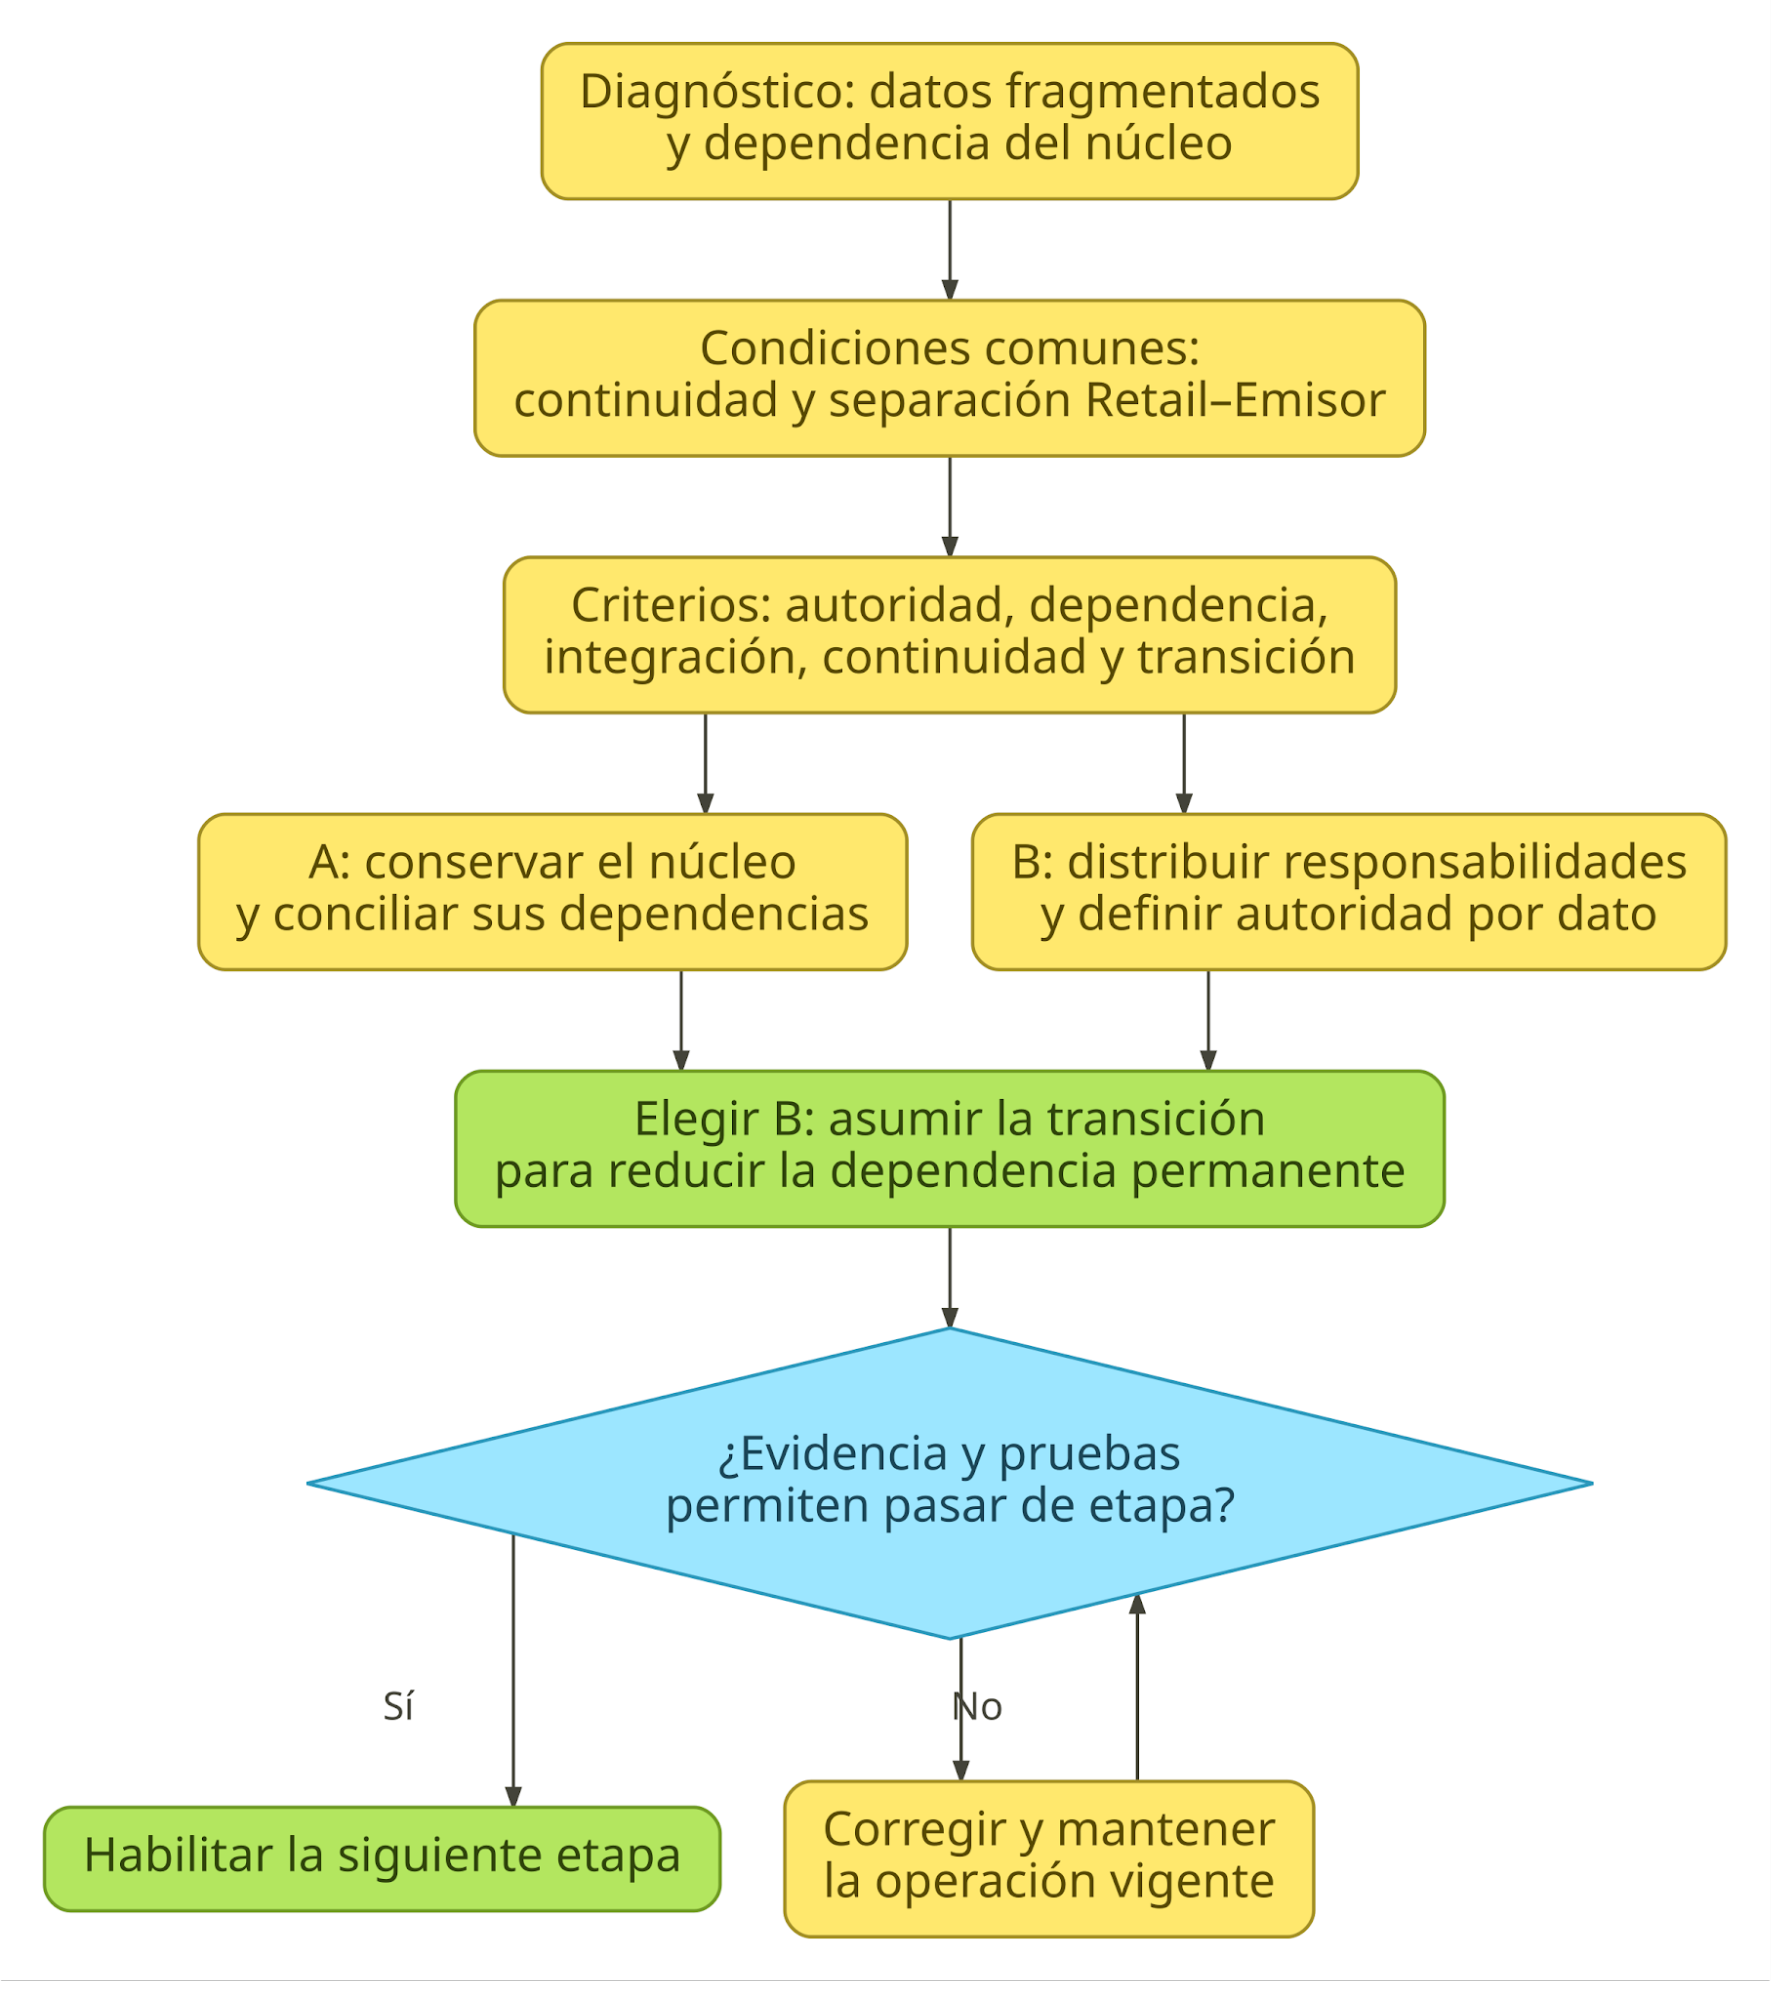
\includegraphics{figuras/sd-03_fig-3-1.png}}\end{center}

{Fuente: elaboración propia; diagrama editable en }{Miro}{.}

{La lectura comienza en el diagnóstico y aplica las mismas condiciones y criterios a las alternativas A y B. La elección acepta el esfuerzo de migración para reducir la dependencia permanente del núcleo. Cada avance requiere evidencia y pruebas; si no las supera, se corrige la transición manteniendo la operación vigente.}

{Del escenario elegido se derivan tres frentes: Retail y Filial emisora conservan sus responsabilidades de negocio y datos; Frontera reúne el control de sus intercambios. La descomposición por áreas y servicios se desarrolla a continuación. La plataforma común y los componentes locales habilitan esa operación y su continuidad.}

{Los actores que intercambian información con la solución corresponden a los grupos identificados en 2.4: clientes y titulares de tarjeta; personal de venta, caja, tiendas y centros de distribución; áreas comerciales y financieras; proveedores, vendedores de marketplace y transportistas. Los organismos fiscalizadores reciben los reportes y antecedentes que les corresponden. La participación de una misma persona en procesos comerciales y financieros no altera la separación de sus datos: cada acceso responde al rol y a la finalidad autorizada.}

{Como se delimitó al comparar las alternativas, ERP/DTE, el WMS principal y la plataforma vigente de marketplace conservan sus responsabilidades e interfaces con los nuevos servicios. El centro de distribución de Concepción entrega registros estructurados mientras se evalúa su incorporación a un WMS. Los sistemas conservados se sitúan fuera del límite de los nuevos servicios funcionales porque mantienen responsabilidades propias (Caso 09, capítulo 5).}

{Comercio electrónico y fidelización se conservan e integran inicialmente para sostener sus canales durante la transición. TI y los responsables de canales y clientes Retail evaluarán desempeño, consistencia, interoperabilidad y separación de datos con las pruebas de la primera etapa. SD-06 programará la decisión de conservar, remediar o sustituir cada plataforma antes de la ola que dependa de ella. Así, su evolución utiliza evidencia de operación y no pospone los resultados exigibles de la primera etapa.}

{Durante la transición del escenario B, el sistema central Retail de 2009 continúa operando hasta que se verifica la transferencia de sus funciones y registros. La plataforma financiera de 2011 convive con el Servicio de originación de crédito, el Servicio de cartera de crédito y el Servicio de evidencia financiera durante la migración por olas de la cartera; el punto de venta de 2014 se sustituye tienda por tienda tras acreditar la operación sin conexión y el retorno. La plataforma de integración sostiene los intercambios de cada ola y permite retirar las conexiones antiguas una vez verificado el nuevo flujo.}

\subsection{3.3.2 Servicios de negocio y autoridad de datos}

{La descomposición sigue la secuencia frente, área y servicio. Cada servicio implementa una capacidad de negocio, custodia sus datos y los expone mediante contratos definidos. La plataforma común habilita su operación. Los códigos siguen la forma frente:área-número: R identifica Retail; F, Filial emisora; M, Mercadería; V, Venta; CL, Relación con el cliente; y C, Crédito. Por ejemplo, F:C-03 identifica el Servicio de evidencia financiera. El Servicio de control de cruces conserva X-01, sin área.}

\subsubsection{Frente Retail}

{Los nueve servicios Retail se agrupan en tres áreas. Mercadería administra la oferta, el suministro y las existencias; Venta coordina pedidos, ventas, comisiones y marketplace; Relación con el cliente gestiona la posventa y la identidad comercial.}

{Área Mercadería. Reúne la oferta comercial, el abastecimiento y las existencias.}

{Servicio de oferta comercial. Administra artículos, atributos, precios, promociones, vigencias y el historial de publicación por canal y de actualización de etiquetas. Incorpora la función de precios y promociones que hoy no existe como sistema. Entrega la oferta vigente a los canales, al Servicio de existencias, al Servicio de pedidos, al Servicio de ventas y al Servicio de marketplace; no calcula reservas ni registra ventas.}

{Servicio de abastecimiento. Administra órdenes, transferencias, propuestas de reposición y recepciones para coordinar proveedores, tiendas y centros de distribución. Consulta la disponibilidad del Servicio de existencias y se integra con ERP/DTE y con el sistema de gestión de almacenes principal. La ejecución física de ubicaciones, preparación y despacho continúa en este último; las planillas de Concepción no pasan a ser una autoridad permanente por el solo hecho de integrarse.}

{Servicio de existencias. Consolida existencias y movimientos por nodo, administra reservas y calcula el disponible comprometible con un margen de confianza por categoría y punto. Registra conteos, ajustes y causas de diferencia. Recibe movimientos del sistema de gestión de almacenes, del punto de venta, del Servicio de abastecimiento y del Servicio de posventa; comunica disponibilidad al Servicio de pedidos, Servicio de marketplace y los canales. El sistema de almacenes conserva la autoridad de ejecución física y ERP/DTE, su registro contable. Los resultados de conteo alimentan la revisión del margen, denominado descuento de seguridad en la operación actual, y permiten priorizar nuevos conteos. Una ayuda de clasificación podrá sugerir la causa de una diferencia con su evidencia; la persona responsable confirma la causa antes de cerrar el ajuste.}

{Área Venta. Reúne los pedidos, las ventas, las comisiones y el gobierno de marketplace.}

{Servicio de pedidos. Administra el ciclo y el estado único del pedido, la fecha prometida y el nodo de preparación elegido por costo total de servir. Solicita la reserva al Servicio de existencias y coordina canales, tiendas, centros de distribución y transportistas hasta el retiro o la entrega. Comparte el estado resultante con el Servicio de comisiones, el Servicio de marketplace y el Servicio de posventa; no reemplaza la ejecución física del sistema de almacenes.}

{Servicio de ventas. Registra ventas, pagos, reversas y registros de caja procedentes del punto de venta y del canal digital, incluidas las operaciones realizadas sin enlace que se sincronizan posteriormente. Concilia esos hechos y entrega la venta confirmada al Servicio de comisiones y al Servicio de posventa. Se integra con ERP/DTE para mantener el estado del documento, mientras ERP/DTE permanece como único emisor tributario.}

{Servicio de comisiones. Aplica reglas auditables para atribuir una venta y su base de comisión al canal, vendedor y tienda que corresponden, incluso cuando una tienda abastece un pedido originado en otro canal. Consume pedidos del Servicio de pedidos y ventas del Servicio de ventas; entrega la base calculada al proceso de remuneraciones que conserva el sistema empresarial. No administra remuneraciones.}

{Servicio de marketplace. Relaciona la plataforma vigente con la oferta, disponibilidad, pedidos, devoluciones y liquidaciones que gestiona Ancoa. Administra las reglas de habilitación y desempeño de vendedores externos y comunica a cada parte el estado que le corresponde. Se apoya en el Servicio de oferta comercial, el Servicio de existencias, el Servicio de pedidos y el Servicio de posventa; no sustituye la plataforma de marketplace ni opera la logística propia de cada vendedor.}

{Área Relación con el cliente. Reúne la posventa y la identificación y fidelización comercial.}

{Servicio de posventa. Abre y resuelve los casos de cambio, devolución, retracto y garantía frente al cliente, con registro de recepción, inspección y destino de cada unidad. Consulta la venta en el Servicio de ventas, informa al Servicio de existencias cuándo una unidad puede volver al disponible y coordina las operaciones de marketplace con su servicio responsable y las notas de crédito con ERP/DTE. La atención al consumidor no se supedita a la conciliación posterior con el vendedor o fabricante.}

{Servicio de clientes Retail. Administra la identificación y deduplicación de clientes, puntos, segmentos, campañas y preferencias dentro de Retail. Integra inicialmente la plataforma vigente bajo separación de datos; su integración definitiva o sustitución se decidirá mediante el mecanismo de primera etapa previsto en 3.3.1 y desarrollado en SD-06. Cualquier solicitud de datos del Emisor se somete al Servicio de control de cruces y a una finalidad y fundamento validados. Saldos, mora, cupos y comportamiento de pago no se incorporan por defecto al perfil comercial.}

\subsubsection{Frente Filial emisora}

{El área Crédito agrupa los tres servicios financieros. Mantiene bajo autoridad de la Filial emisora las decisiones crediticias, la cartera y la evidencia contractual. Sus resultados se entregan a Retail conforme a la finalidad y autorización del intercambio.}

{Servicio de originación de crédito. Administra solicitudes, evaluaciones, cupos, decisiones y autorizaciones de crédito iniciadas en los canales habilitados. Antes de confirmar una apertura exige la información y evidencia custodiadas por el Servicio de evidencia financiera y comunica al Servicio de ventas el resultado necesario para la venta. No origina tarjetas nuevas ni amplía cupos durante una pérdida de enlace.}

{Servicio de cartera de crédito. Administra cuentas, saldos, cuotas, pagos, mora, cobranza y modificaciones de condiciones. Consulta al Servicio de evidencia financiera antes de confirmar una repactación y conserva la trazabilidad de su expediente. La cartera de la plataforma actual se transfiere por olas conciliadas, conforme a 3.2; sus saldos no se publican en el Servicio de clientes Retail ni en perfiles comerciales.}

{Servicio de evidencia financiera. Custodia la versión de la información precontractual entregada, la aceptación, el consentimiento y la evidencia de firma vinculados a cada operación. El Servicio de originación de crédito y el Servicio de cartera de crédito consultan este servicio para impedir una originación o repactación sin evidencia suficiente. Asegura integridad, acceso controlado y recuperación durante el plazo exigido; no administra saldos ni decisiones de crédito.}

\subsubsection{Frente Frontera}

{Este frente contiene el Servicio de control de cruces y no se subdivide en áreas. El servicio es responsable de las políticas, las decisiones de autorización y su evidencia. Los datos comerciales y crediticios permanecen bajo autoridad de los servicios que los producen; los controles del intercambio se aplican en sus extremos.}


{Servicio de control de cruces. Define y versiona las condiciones de cada intercambio: finalidad, fundamento, solicitante, destinatario y datos mínimos. El ámbito que entrega verifica la política antes de liberar información; el receptor limita su uso a la finalidad aprobada. Ambos extremos registran autorizaciones, denegaciones y versión de política. El servicio se entrega en la primera etapa mediante catálogo de flujos, contratos, reglas aplicadas, bitácora y pruebas de minimización, rechazo y rutas alternativas. No crea un maestro único de clientes ni habilita atributos financieros para Marketing.}

{La plataforma común conecta servicios y sistemas conservados mediante contratos y adaptadores para intercambiar solicitudes, resultados y hechos de negocio. Registra el envío y su resultado para detectar fallas y apoyar la conciliación. La identidad y los permisos distinguen personas, roles y ámbitos; la observabilidad permite a TI detectar retrasos. Estas funciones habilitan las responsabilidades del catálogo y no sustituyen la autoridad del dato ni la autorización de un cruce.}

{La capacidad analítica de la plataforma ofrece tableros e informes de autoservicio sobre registros publicados por sus servicios responsables, sin cargar consultas analíticas sobre las bases transaccionales. Mantiene espacios de datos, modelos de consulta y permisos separados para Retail y la Filial emisora. La consulta de detalle, la exportación y el envío programado respetan esa separación. Un conjunto de datos que requiera información de ambos ámbitos solo podrá incorporarse tras definir y aprobar su finalidad, fundamento, campos mínimos y responsables conforme al Servicio de control de cruces; la existencia de una interfaz común no concede acceso entre ámbitos. El catálogo y el linaje de indicadores permitirán reconstruir qué fuentes y transformaciones respaldan cada resultado. Su diseño físico y sus políticas se precisarán en los subdocumentos de arquitectura y datos.}

{El punto de venta (POS) y los componentes locales mantienen las funciones de tienda durante una pérdida de enlace. Conservan las condiciones vigentes y las operaciones que deberán conciliarse al recuperar la conexión; el Servicio de ventas recibe ese registro. La interfaz del nuevo POS distinguirá la venta Retail de la sesión bajo rol financiero y hará visibles al personal los estados de disponibilidad, precio y sincronización necesarios para atender excepciones. ERP/DTE mantiene la responsabilidad tributaria y el WMS la ejecución física. La continuidad y sus límites se explican en 3.4.5; los mecanismos técnicos se desarrollarán en arquitectura.}

{En la primera etapa se entregan el Servicio de oferta comercial, el Servicio de existencias, el Servicio de ventas, el Servicio de originación de crédito, el Servicio de evidencia financiera y el Servicio de control de cruces, junto con la plataforma común y el nuevo punto de venta. El Servicio de cartera de crédito se migra por olas en ambas etapas; los demás servicios Retail se incorporan en la segunda. Esta distribución conserva los hitos de 3.2.}

\subsubsection{Vistas de contexto y relaciones principales}

{La Figura 3.2 presenta el contexto general del escenario B. Las Figuras 3.3, 3.4 y 3.5 amplían las relaciones de Retail, del Emisor y los escenarios de intercambio. Los rótulos abrevian los nombres del catálogo y omiten el prefijo «Servicio de»; los códigos R/F/X se mantienen en el alcance y los entregables. Las flechas opuestas representan solicitudes y respuestas. Los contratos y mecanismos de transporte se definirán en la arquitectura lógica.}

{Figura 3.2. Contexto de la solución propuesta para Ancoa (escenario B).}

\begin{center}\pandocbounded{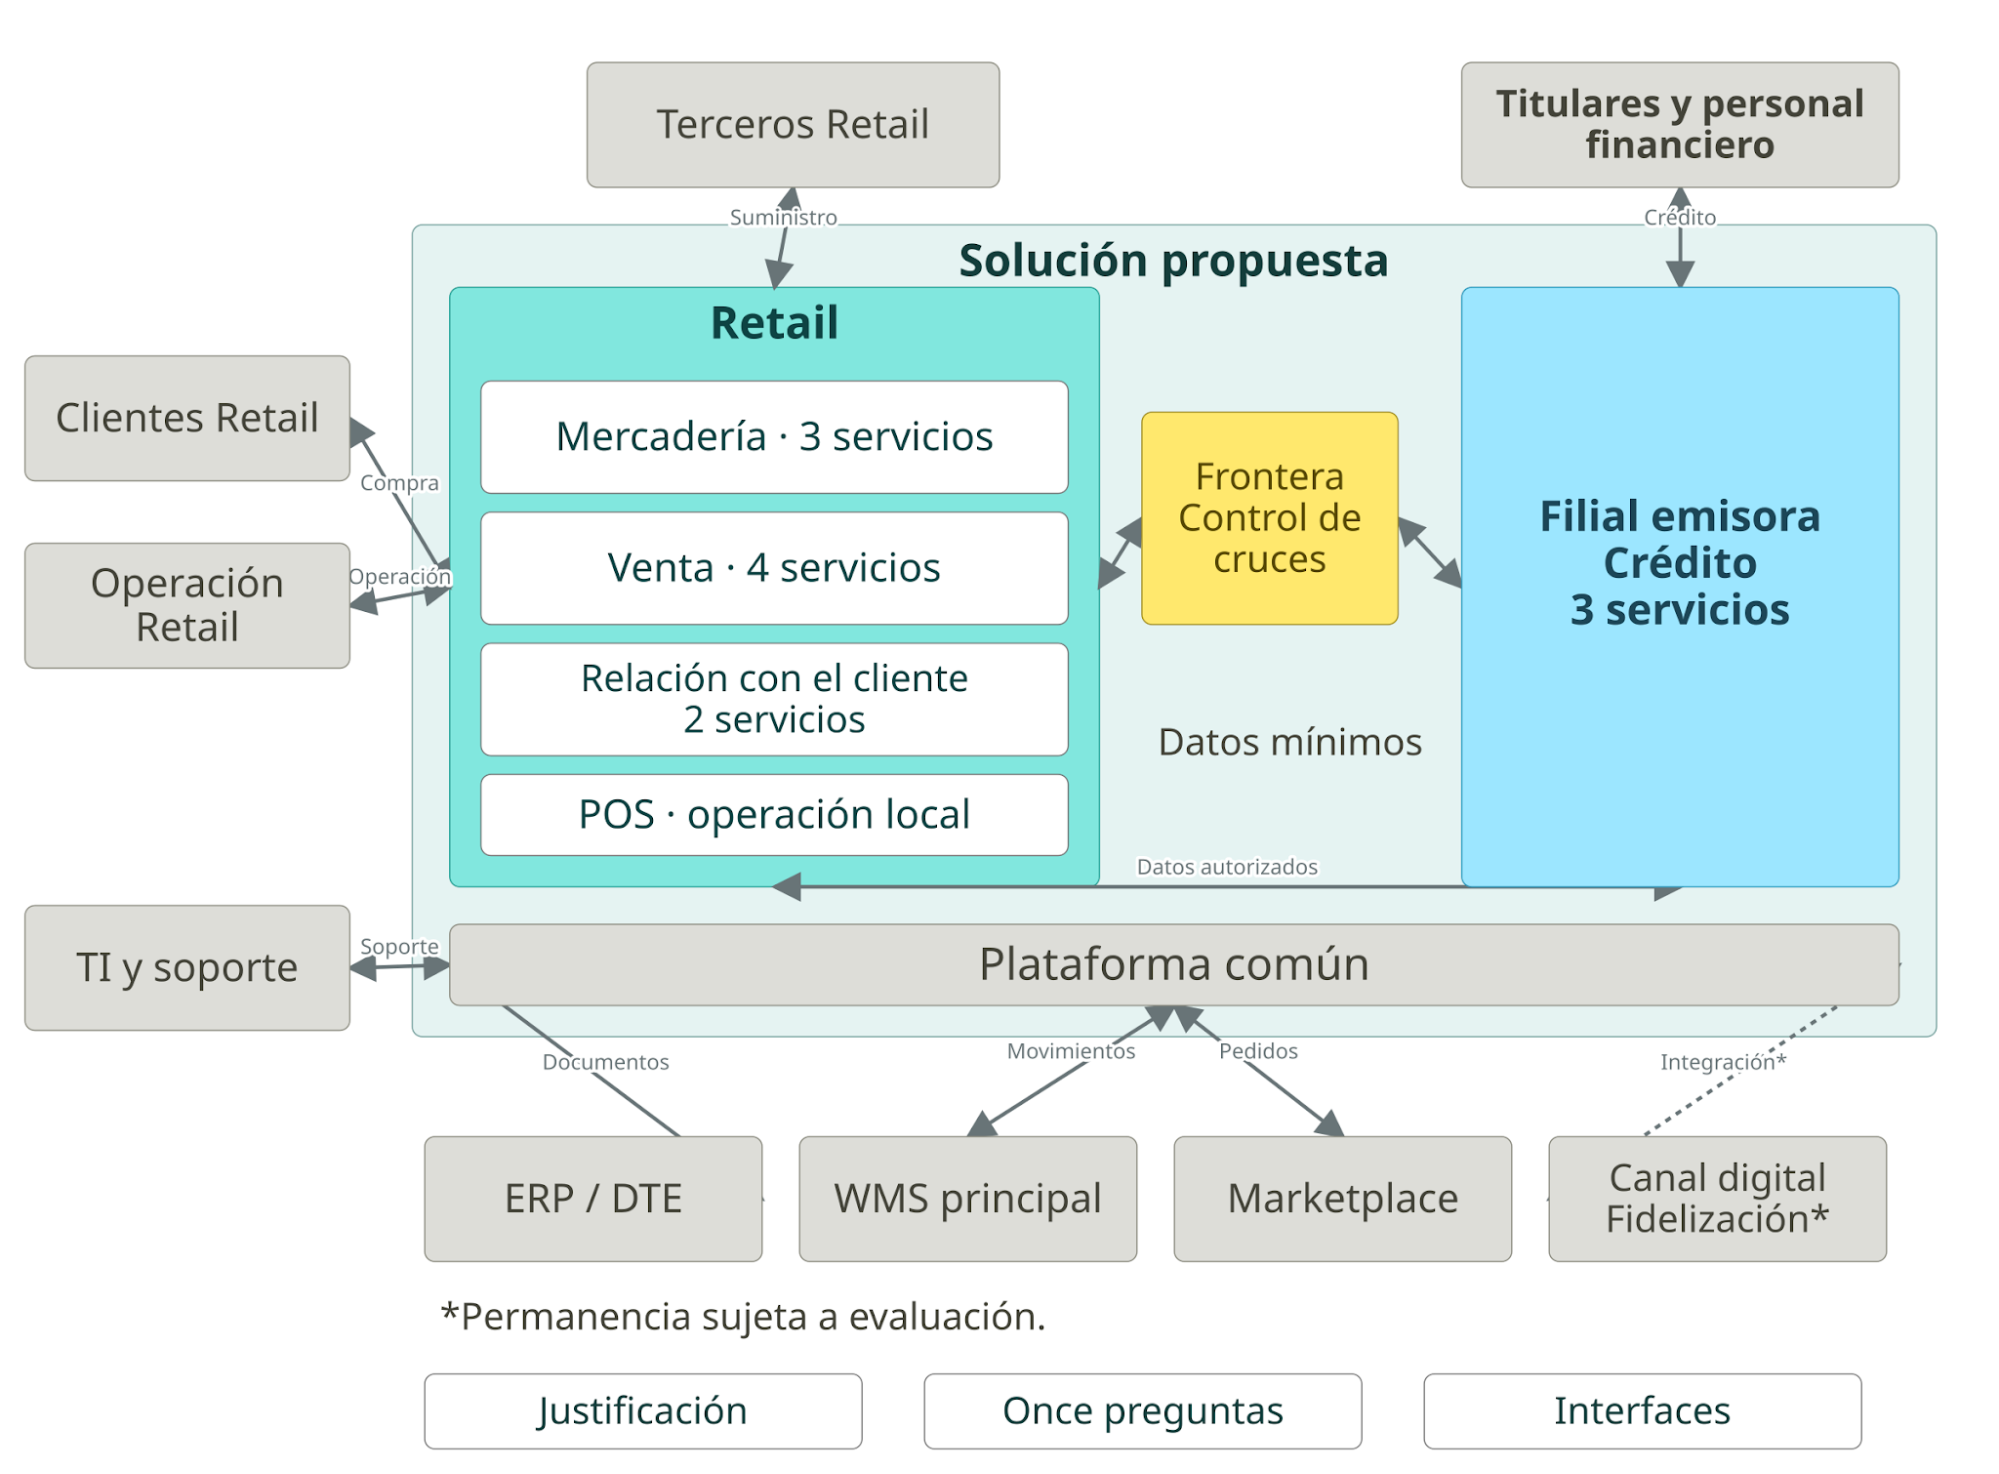
\includegraphics{figuras/sd-03_fig-3-2.png}}\end{center}

{Fuente: elaboración propia a partir del Caso 09, capítulo 5, y del alcance de SD-03.}

{La Figura 3.2 muestra los tres frentes y el límite de la solución. Retail agrupa nueve servicios en Mercadería, Venta y Relación con el cliente; la Filial emisora reúne tres en Crédito. Frontera contiene el Servicio de control de cruces. Las plataformas externas se conservan o evalúan según el alcance ya expuesto.}

{El Servicio de control de cruces se representa sobre la frontera porque autoriza, minimiza y audita el uso de datos entre los negocios. La plataforma de integración ofrece transporte y adaptadores. Los controles y el registro de las decisiones se aplican en los extremos del intercambio; esta vista no fija un despliegue físico único.}

{Las flechas de la vista general son familias de relación, no contratos implantados. Las vistas siguientes muestran quién solicita información, quién responde y qué datos permanecen bajo autoridad de cada ámbito. El mapa de las catorce interfaces existentes se levantará durante la primera etapa.}

{La Figura 3.3 amplía el ámbito Retail. Muestra los nueve servicios comerciales, sus canales y las plataformas que permanecen integradas. La lectura sigue el ciclo desde la oferta y la disponibilidad hasta el pedido, la venta y la atención posterior.}

{Figura 3.3. Servicios Retail y relaciones con canales y plataformas conservadas.}

\begin{center}\pandocbounded{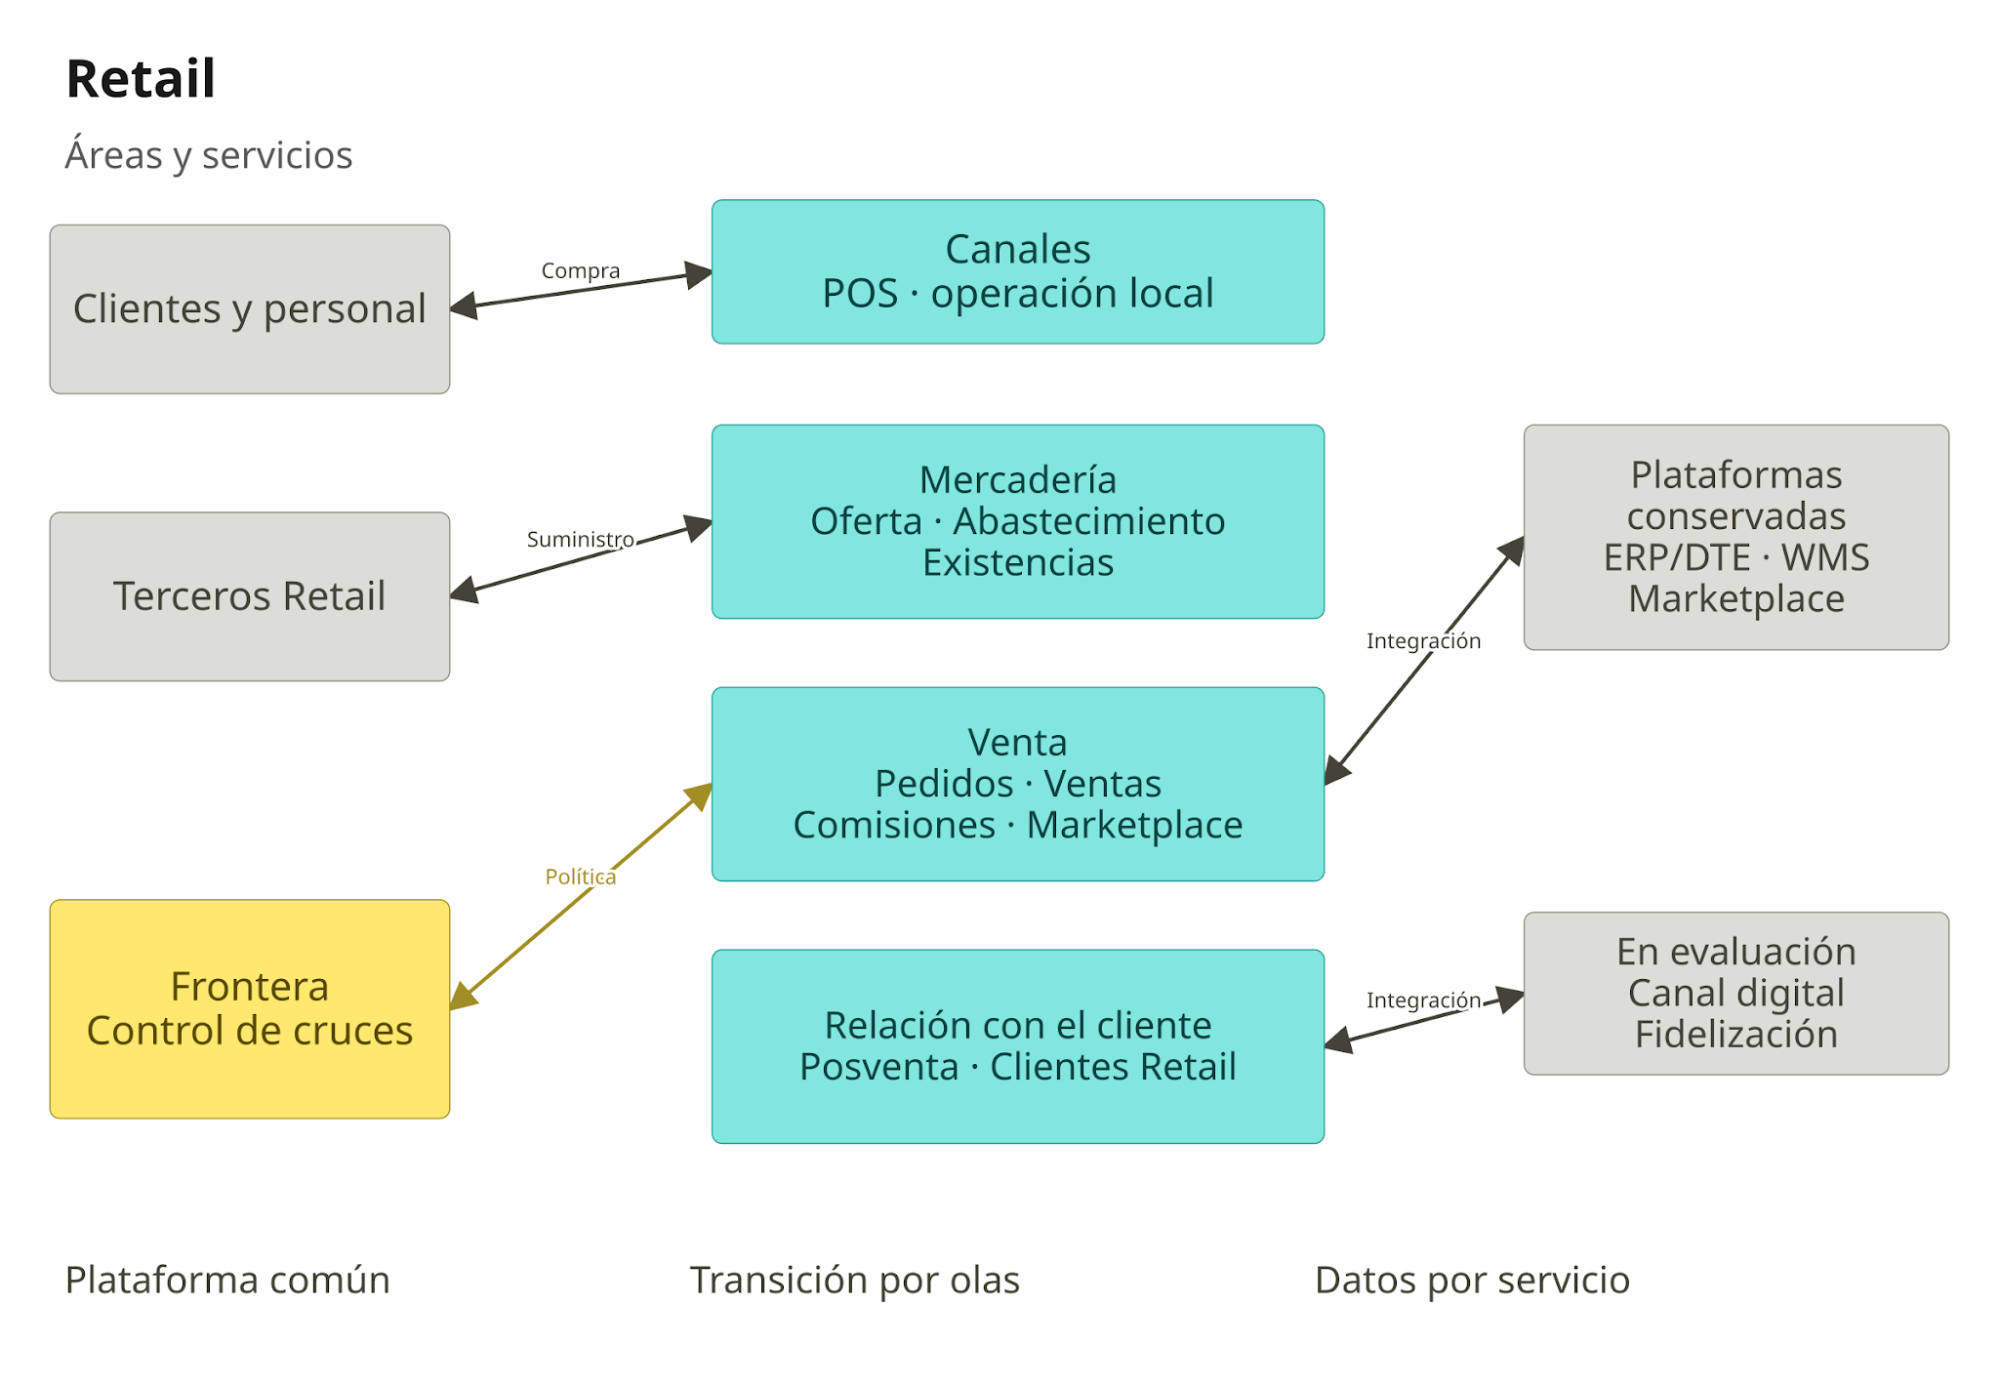
\includegraphics{figuras/sd-03_fig-3-3.png}}\end{center}

{Fuente: elaboración propia a partir del Caso 09, capítulos 4 y 5, y del alcance de SD-03.}

{La Figura 3.3 vincula las áreas Retail con sus canales y plataformas. Las conexiones amarillas de las Figuras 3.3 y 3.4 representan la aplicación de la política de cruces en cada ámbito; la compra se desarrolla en la Figura 3.5. Estas relaciones de control no fijan una ruta física única.}

{La Figura 3.4 amplía el ámbito del Emisor. Presenta la evaluación y autorización de crédito, la administración de cartera y la custodia de evidencia financiera, junto con el acceso de titulares y personal autorizado.}

{Figura 3.4. Servicios del Emisor y custodia de decisión y evidencia financiera.}

\begin{center}\pandocbounded{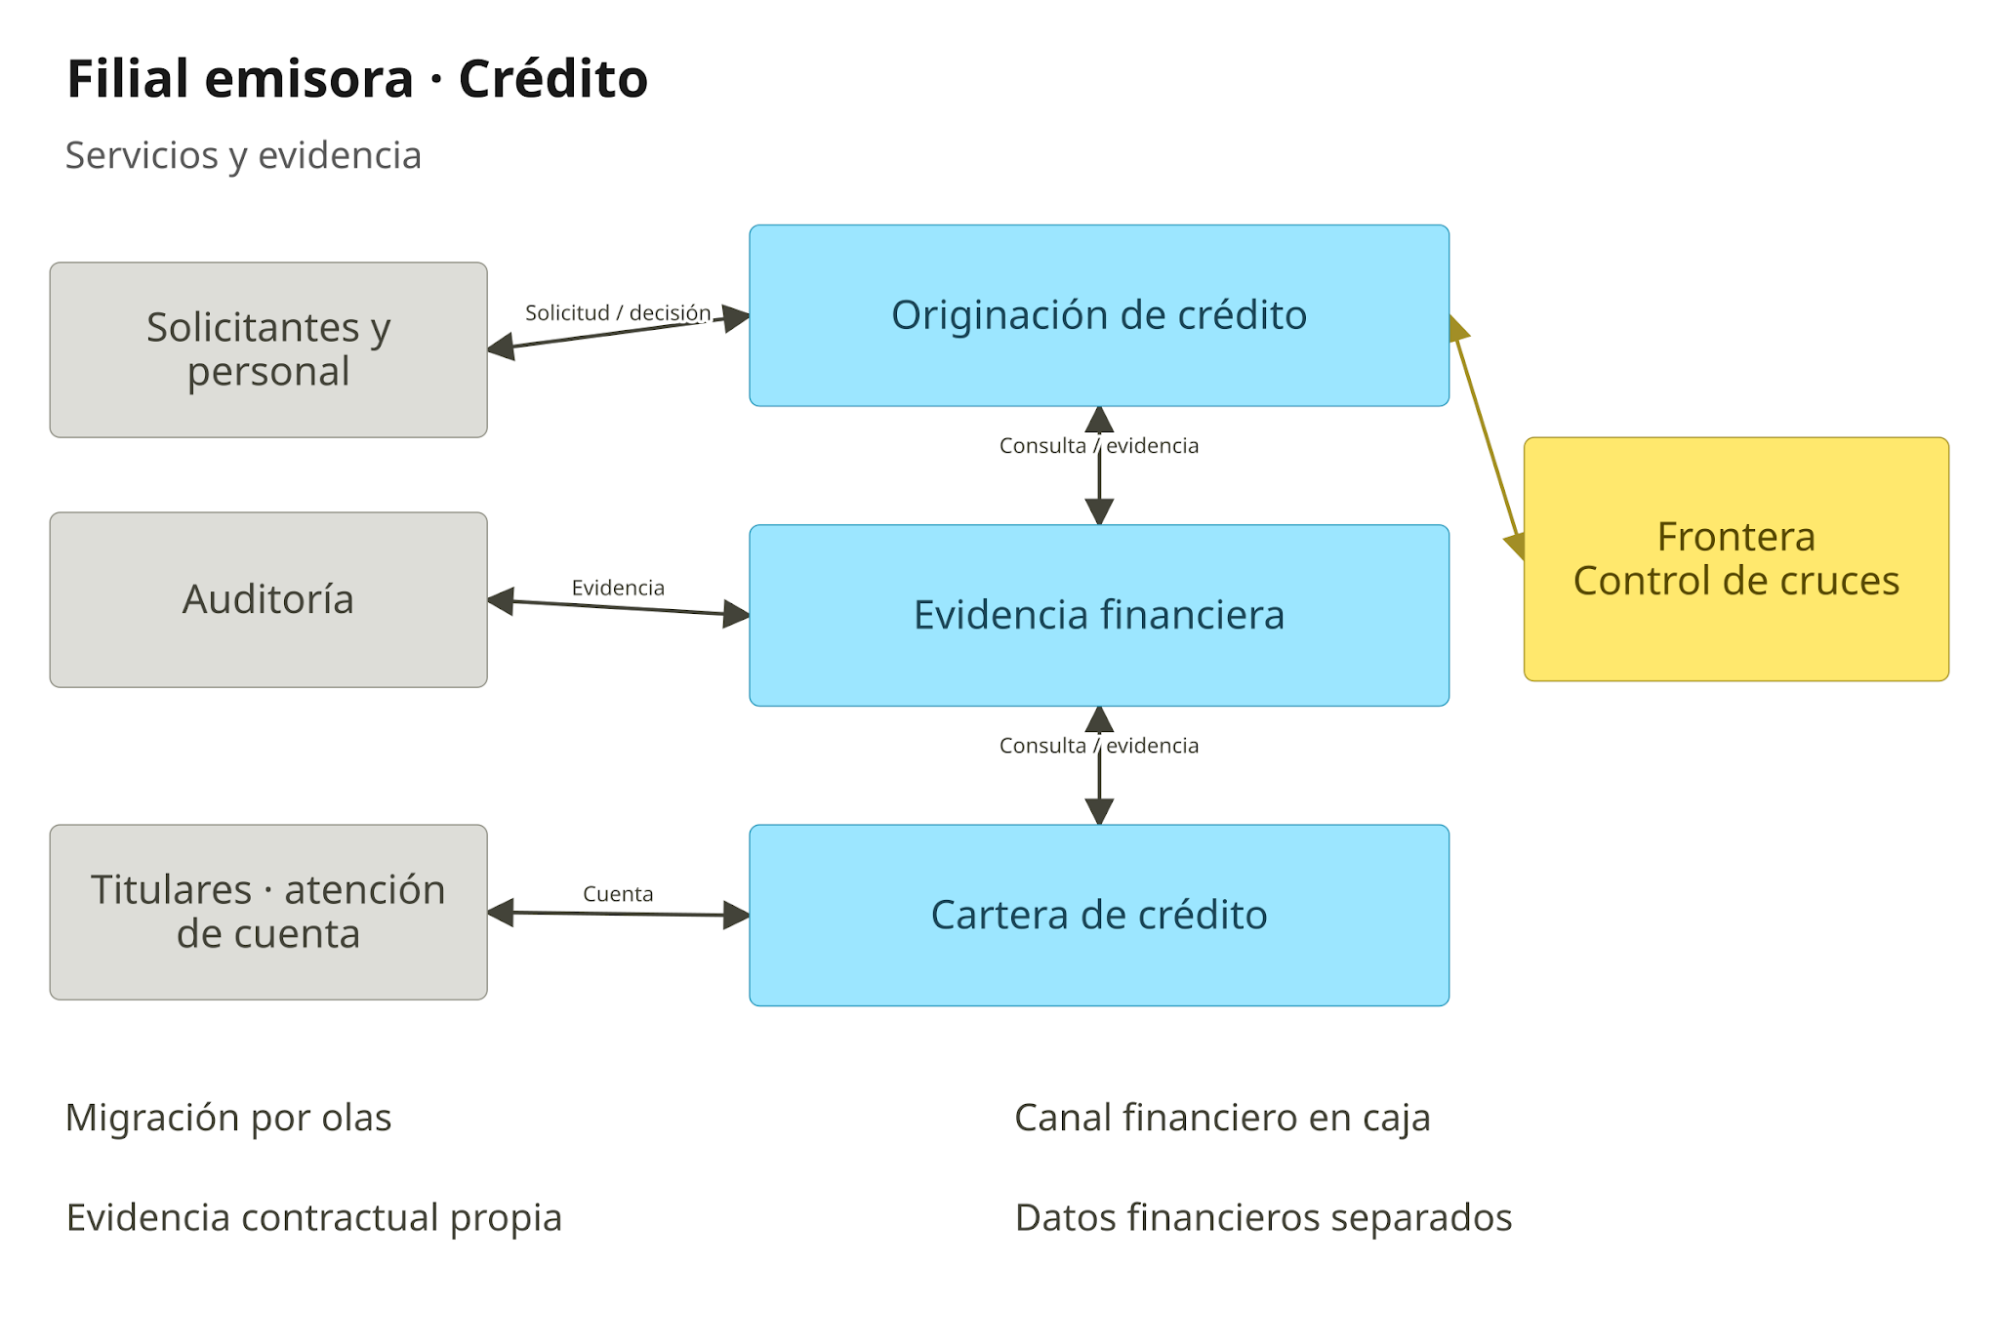
\includegraphics{figuras/sd-03_fig-3-4.png}}\end{center}

{Fuente: elaboración propia a partir del Caso 09, capítulos 4, 5 y 9, y del alcance de SD-03.}

{La figura separa decisión, administración de deuda y prueba contractual. Originación y repactación consultan la evidencia de la información entregada y aceptada antes de confirmarse. La plataforma financiera de 2011 participa en la migración por olas hasta su retiro; la falta de enlace no autoriza nuevas tarjetas ni aumentos de cupo.}

{La Figura 3.5 reúne operaciones en las que podría cruzarse información entre Retail y Emisor, además de una solicitud que debe rechazarse. Presenta compra con tarjeta propia y reversa con sus respuestas; también muestra una originación iniciada en caja, que puede permanecer íntegramente bajo rol financiero, y la venta local durante desconexión, sin consulta al Emisor.}

{Figura 3.5. Escenarios y límites del intercambio Retail--Emisor.}

\begin{center}\pandocbounded{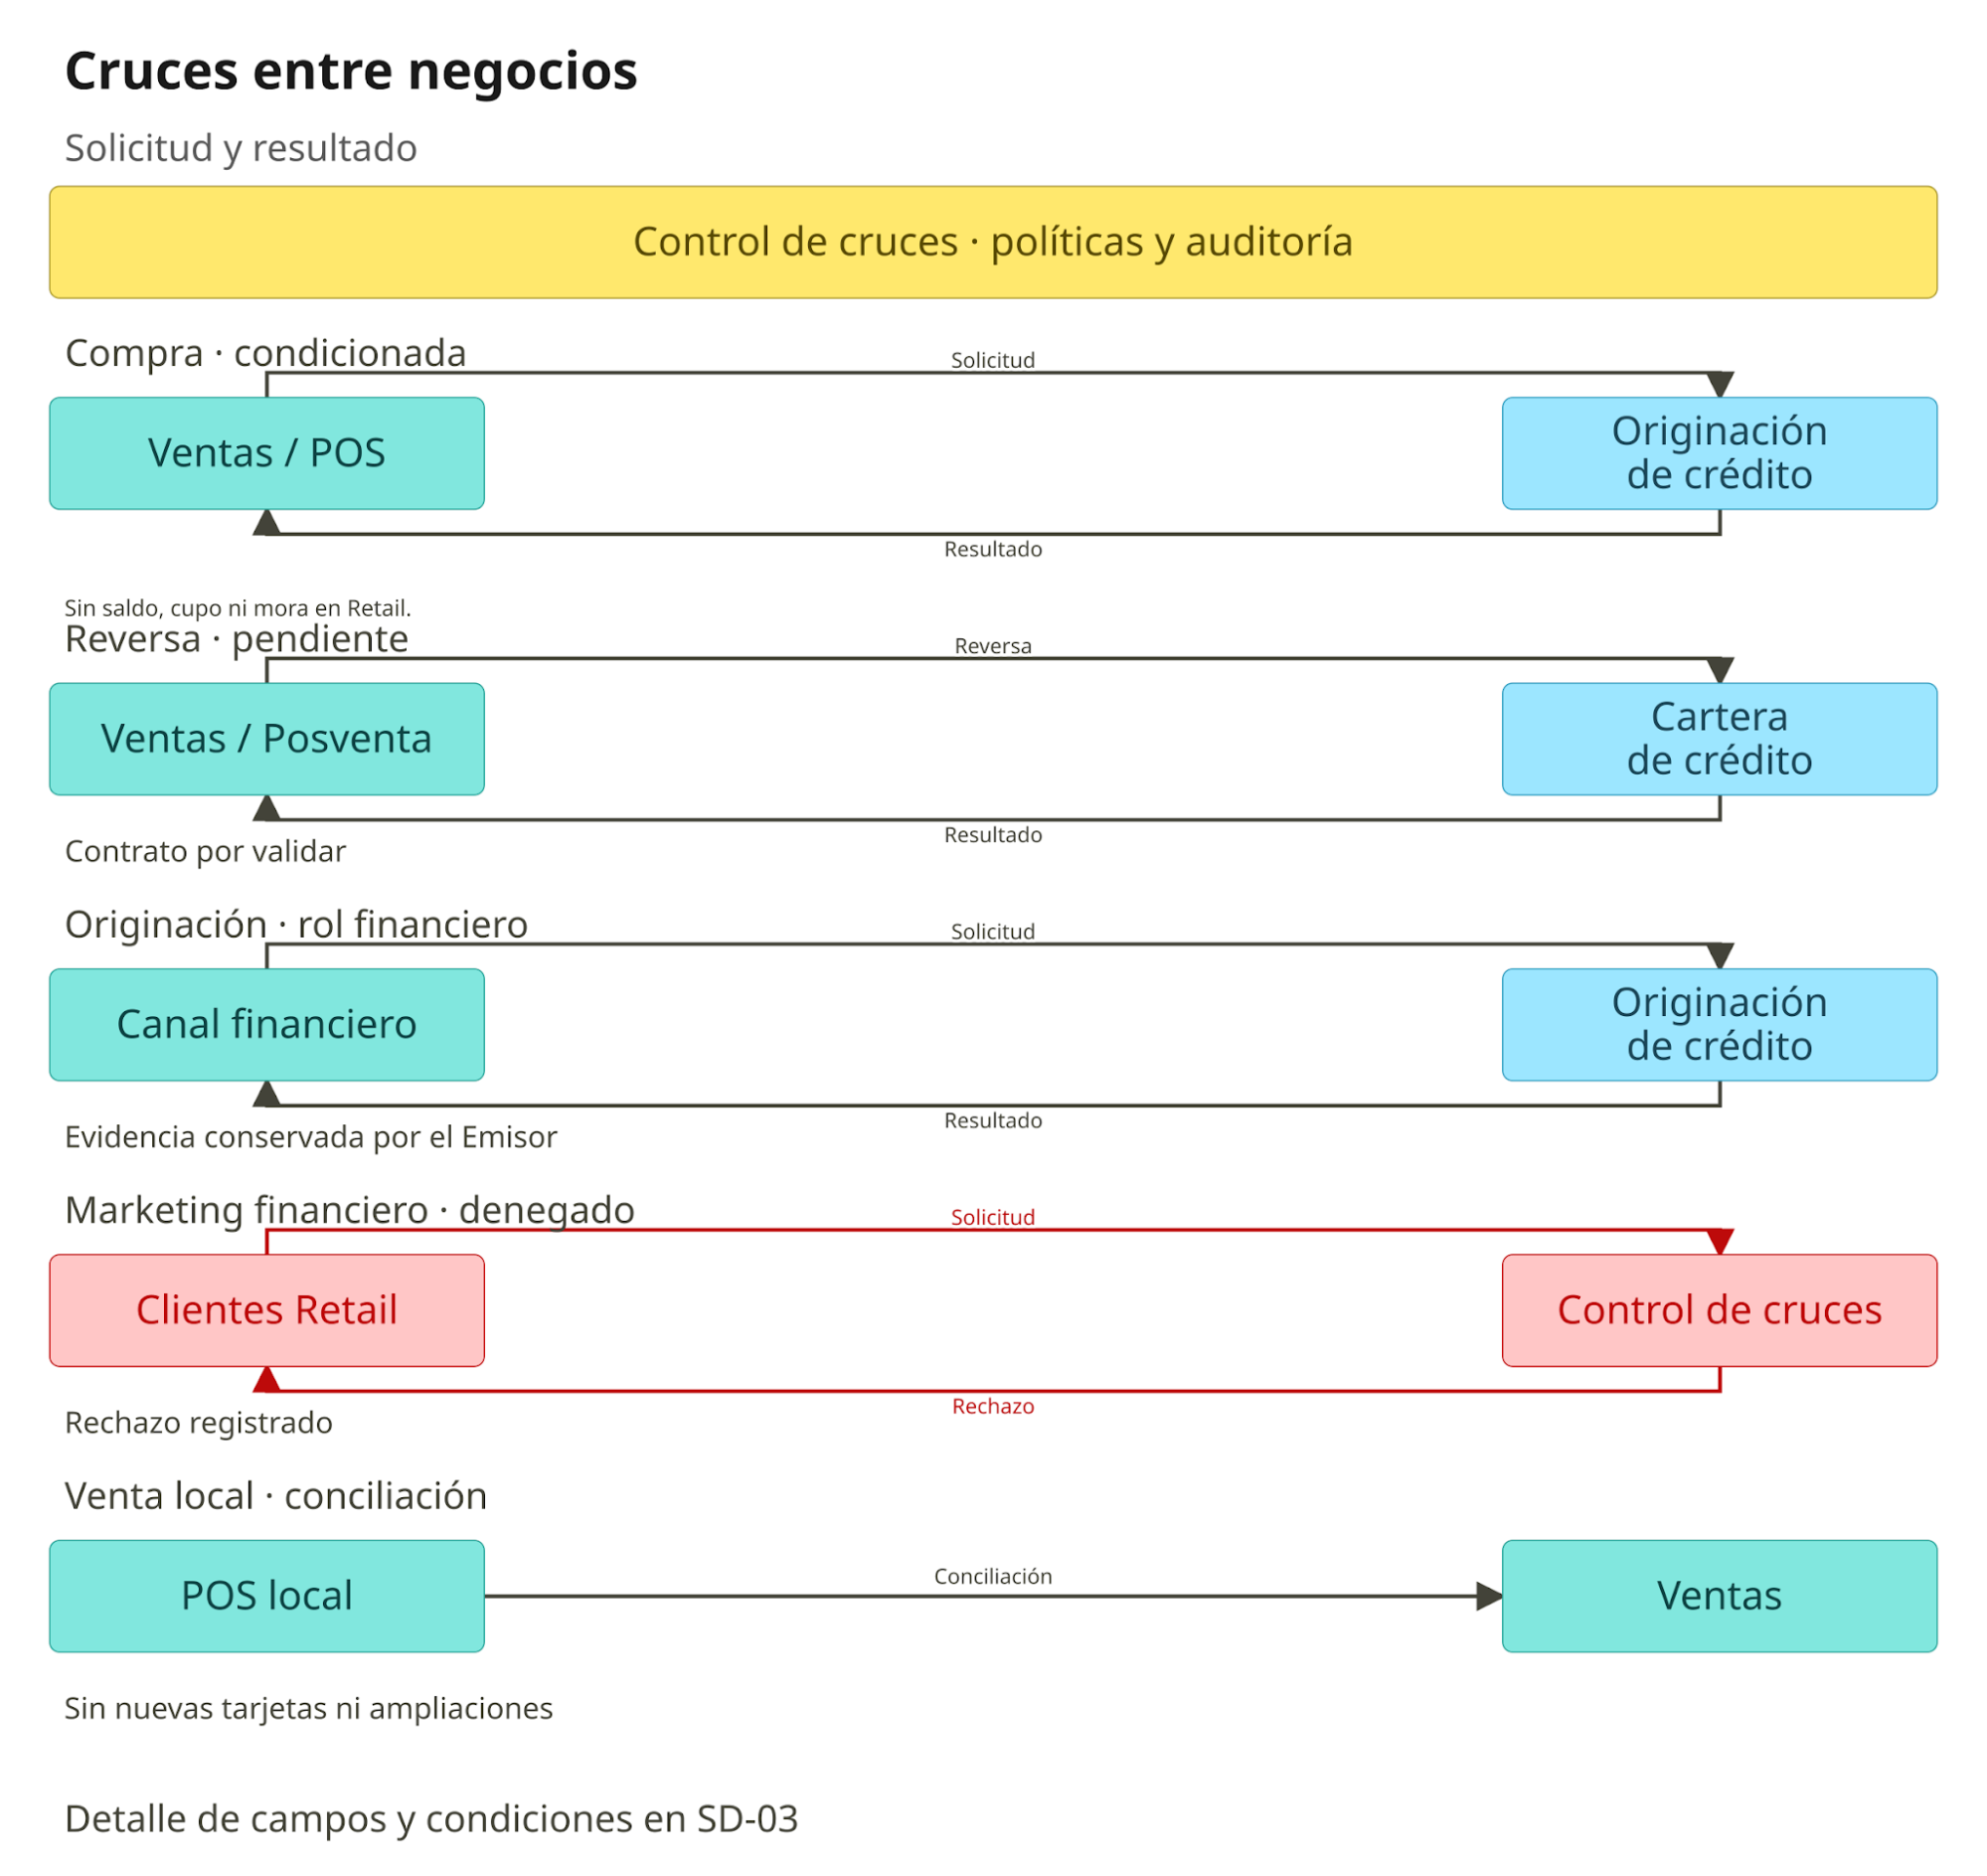
\includegraphics{figuras/sd-03_fig-3-5.png}}\end{center}

{Fuente: elaboración propia a partir del Caso 09, 9.10 y 10.1, y del alcance de SD-03.}

{La compra con tarjeta propia devuelve a Retail solo el resultado de esa venta; saldo y mora permanecen en el Emisor. La reversa es una propuesta cuya necesidad y contrato aún deben acreditarse. Marketing recibe una denegación sin datos de pago. La originación en caja exige evidencia precontractual distinta de la autorización de compra; si el canal actúa bajo el rol del Emisor, su ubicación en una tienda no crea un cruce hacia Retail. Durante la desconexión, el POS registra la venta y la concilia al volver el enlace; una compra contra autorización previa exige reglas específicas y no permite originar tarjetas ni ampliar cupos. El control transversal registra la decisión de intercambio y el Servicio de evidencia financiera conserva la prueba contractual.}

\subsubsection{Gobierno de los intercambios Retail--Emisor}

{La Figura 3.5 delimita las operaciones; esta sección define sus condiciones de habilitación. Cada intercambio requiere finalidad, fundamento, responsable, destinatario y datos mínimos registrados en una ficha aprobada. Retail y Emisor aplican la política en sus extremos y conservan evidencia de permitir o denegar. Una aceptación contractual de crédito no autoriza por sí sola el uso comercial de información de deuda.}

{Fundamento y transición normativa. A octubre de 2026 rige la Ley N.º 19.628 en su texto vigente, que exige autorización legal o consentimiento para el tratamiento y limita la comunicación de datos económicos (arts. 4 y 17). La Ley N.º 21.719 modifica ese régimen desde el 1 de diciembre de 2026 e incorpora exigencias expresas de licitud, finalidad, proporcionalidad, seguridad y responsabilidad; el diseño de la etapa operativa deberá cumplirlo. La Ley N.º 19.496 exige información y condiciones claras en los contratos financieros (arts. 17 B y siguientes). La Circular N.º 1 de la CMF para emisores no bancarios establece resguardos de riesgo operacional, continuidad y seguridad de la información. Estas normas no determinan por sí solas que Retail pueda recibir comportamiento de pago ni el plazo de cada bitácora del Servicio de control de cruces.}

{Las Bases del Caso 09 exigen una frontera documentada, implementada y auditable (9.10 y restricción 10.1), describen el cruce indebido de fidelización con pago y fijan retención contractual por categoría en RT-05.10. El Servicio de control de cruces acredita la decisión de compartir y el uso permitido; el Servicio de evidencia financiera custodia por separado la información precontractual, aceptación, firma y grabaciones de originación y repactación. Su evidencia no reemplaza el registro del intercambio ni viceversa.}

{La Tabla 3.6 relaciona separación, licitud, acceso y retención con responsable, control y evidencia.}

Tabla 3.6: Obligación, responsable, control y evidencia del Servicio de control de cruces.


\begin{longtable}{@{}p{0.19\linewidth}p{0.20\linewidth}p{0.27\linewidth}p{0.25\linewidth}@{}}
\toprule\noalign{}
\endhead
\bottomrule\noalign{}
\endlastfoot
{Exigencia / fuente} & {Responsable} & {Control X-01} & {Entregable y prueba} \\
{Separación auditable; Caso 09, 9.10 y 10.1} & {Retail y Emisor; cumplimiento aprueba} & {Catálogo por finalidad; denegar rutas no inventariadas} & {Matriz, políticas versionadas, prueba de desvío y bitácora} \\
{Licitud, finalidad y mínimos; Ley 19.628, arts. 4 y 17; Ley 21.719 desde 01-12-2026} & {Responsable del dato en cada entidad; asesoría jurídica valida fundamento} & {Ficha aprobada, campos mínimos y bloqueo de uso secundario} & {Ficha jurídica por flujo, respuesta limitada y pruebas de denegación} \\
{Acceso y seguridad; Ley 21.719 y Circular 1 CMF; RT-11.11} & {Emisor controla salida; Retail controla recepción; TI opera} & {Identidad, rol, autorización, esquema, cifrado y registro} & {Contratos, controles en ambos extremos y evidencia de acceso} \\
{Retención; Caso 09 RT-05.10 y plazo jurídico aplicable} & {Dueño del registro; F:C-03 custodia evidencia contractual} & {Separar bitácora de cruce de expediente financiero; calendario aprobado} & {Prueba de recuperación, purga y trazabilidad; crédito: plazo + 6 años según Bases} \\
\end{longtable}

{Fuente: elaboración propia a partir del Caso 09, 9.10 y RT-05.10; Bases Transversales, RT-11.11; y legislación citada en referencias.}

{La Tabla 3.6 relaciona los controles que deberán aplicarse y probarse en ambos ámbitos. El plazo de la evidencia contractual no se traslada automáticamente a la bitácora de intercambio: esta requiere una regla propia, según su categoría y fundamento.}

{La matriz siguiente distingue compra, reversa y solicitud de Marketing. Cada operación se separa en solicitud y respuesta cuando corresponde. Son intercambios propuestos, no un inventario de las catorce interfaces actuales. La originación en caja puede operar bajo el rol financiero; la venta sin enlace no consulta al Emisor durante la desconexión.}

{La Tabla 3.7 compara los cruces por dirección, finalidad, autoridad, condición y estado. Ventas/POS corresponde al Servicio de ventas y su canal; Crédito, al Servicio de originación de crédito; Cartera, al Servicio de cartera de crédito; y control, al Servicio de control de cruces.}

Tabla 3.7: Escenarios de intercambio Retail--Emisor y condiciones de habilitación.


\begin{longtable}{@{}p{0.18\linewidth}p{0.18\linewidth}p{0.18\linewidth}p{0.18\linewidth}p{0.18\linewidth}@{}}
\toprule\noalign{}
\endhead
\bottomrule\noalign{}
\endlastfoot
{Operación / dirección} & {Finalidad y mínimos} & {Autoridad / uso} & {Condición} & {Estado / evidencia} \\
{Compra: Ventas/POS {[}R:V-02{]} → Crédito {[}F:C-01{]}} & {Autorizar importe; ref., monto, medio} & {Decide Emisor; usa Retail} & {Ficha y contrato aprobados} & {Condicionado; bitácora} \\
{Compra: Crédito {[}F:C-01{]} → Ventas/POS {[}R:V-02{]}} & {Decisión, referencia y vigencia} & {Emisor decide; Retail cierra venta} & {Misma operación autorizada} & {Condicionado; sin deuda} \\
{Pago/reversa: Ventas {[}R:V-02{]} → Cartera {[}F:C-02{]}} & {Hecho comercial; ref., monto, fecha} & {Retail origina; Emisor concilia} & {Necesidad y contrato por acreditar} & {Cerrado hasta aprobación} \\
{Reversa: Cartera {[}F:C-02{]} → Ventas/Posventa {[}R:V-02 / R:CL-01{]}} & {Resultado; referencia y estado} & {Emisor decide; Retail atiende} & {Acceso por transacción} & {Cerrado hasta aprobación} \\
{Marketing → control de cruces} & {Solicitud de perfil con datos de pago} & {Emisor conserva; Retail no recibe} & {Sin fundamento acreditado} & {Denegado; intento registrado} \\
\end{longtable}

{Fuente: elaboración propia a partir del Caso 09, capítulos 4 y 9, y del alcance propuesto en SD-03.}

{La Tabla 3.7 delimita los intercambios habilitables y aquellos que permanecen cerrados. La aprobación de la ficha, su contrato y las pruebas de bloqueo preceden a la activación de cada flujo; el registro deberá permitir demostrar que la operación respetó el límite autorizado.}


\section{3.4 Explicación de la Solución}

{Los recorridos siguientes responden a las brechas de disponibilidad, precio, trazabilidad de pedidos y crédito identificadas en el capítulo 2. Explican cómo intervienen los servicios representados en las Figuras 3.2 a 3.5 y cómo se comprobarán las metas de 3.2.}

\subsection{3.4.1 La promesa de existencia}

{Hoy un cliente puede comprar una unidad que figura disponible y recibir después una cancelación: el conteo físico, la venta en tienda, las reservas digitales y la preparación en almacén no llegan al mismo registro con la misma oportunidad. Las diferencias en el 12,4 \% de las referencias auditadas y las cancelaciones de 1,9 \% anual y 2,7 \% en el evento (Caso 09, capítulos 4 y 9) exigen distinguir la existencia registrada de las unidades que pueden comprometerse con confianza.}

{Con las autoridades y fuentes de movimiento definidas en 3.3, el Servicio de existencias calcula el disponible comprometible (ATP) por categoría y nodo. El cálculo descuenta reservas y compromisos de la existencia conciliada y aplica un margen de confianza por categoría y nodo, cuya calibración y documentación deben completarse antes de habilitar la publicación comprometible. La reserva solicitada por el Servicio de pedidos se confirma o libera según avance la operación y su vigencia; esta secuencia permite reconstruir qué cantidad respaldó la promesa.}

{El descuento de seguridad que se aplica hoy a la existencia publicada es un número fijo definido en 2019, sin revisión acreditada (Caso 09, capítulo 8). La calibración propuesta partirá del historial depurado de conteos, ventas, movimientos, reservas y quiebres. Un modelo predictivo podrá estimar el riesgo y la magnitud de una discrepancia por referencia, ubicación y período para priorizar conteos y aportar evidencia al margen por categoría y nodo. El valor aplicado seguirá siendo un parámetro aprobado y trazable del Servicio de existencias. Se compararán cancelaciones por falta de existencia y unidades retenidas por el margen frente a la regla de referencia; si el modelo no supera esa regla o no hay datos suficientes, se mantendrá la parametrización supervisada.}

{El conteo registra la diferencia observada y abre su investigación. Una segunda capacidad podrá sugerir la causa probable entre pérdida física, daño no dado de baja, error de recepción, unidad mal ubicada, devolución mal reintegrada y error de digitación, acompañada por las señales que fundamentan la sugerencia. Prevención de Pérdidas o el responsable autorizado verificará la evidencia y confirmará la causa antes del ajuste. La evaluación distinguirá los conteos priorizados de una muestra aleatoria o estratificada, para que la selección por riesgo no distorsione la medición de la exactitud general. Se medirán las diferencias relevantes detectadas por cada cien conteos, el tiempo hasta confirmar una causa y el desempeño de la clasificación por causa; las líneas base y metas se fijarán tras perfilar los registros disponibles.}

{Si falta confirmación de disponibilidad antes del cobro, el canal informa la indisponibilidad y no cobra la unidad, conforme al Caso 09, capítulo 18. Una reserva o pedido abierto no se presenta como entrega confirmada cuando esa comprobación ha fallado. Si la diferencia se detecta después, el responsable de pedidos conserva el historial de la promesa, comunica la incidencia y coordina su resolución con posventa. La regla de resolución deberá precisar la alternativa ofrecida al cliente y el tratamiento del cobro, la reserva y el pedido antes de habilitar ese recorrido.}

{El piloto compara exactitud y cancelaciones antes y después, por categoría y nodo y durante el evento anual. La disponibilidad publicada deberá actualizarse dentro de 30 segundos tras una venta (Caso 09, RT-05.29). La aceptación contrastará además las metas de 3.2: diferencia de inventario inferior al 2 \%, cancelaciones anuales inferiores al 0,3 \% y ninguna cancelación por falta de existencia durante el evento.}

{El esfuerzo del ATP comprende conteos cíclicos, depuración y conciliación de movimientos, reservas, publicación y pruebas de máxima demanda. Un margen mayor reduce el riesgo de prometer unidades inexistentes, pero restringe la venta; su evaluación comparará ambas consecuencias en el piloto. La memoria de capacidad deberá derivar la concurrencia, las transacciones y consultas por segundo, el volumen de datos y su crecimiento de la volumetría del Caso 09, numerales 14.1 y 14.2, distinguiendo el evento digital de la campaña presencial. Relacionará estos resultados con las tareas de la EDT, el personal de conteo y las pruebas en Preproducción a 1,5 veces el peak declarado, además del estrés hasta el punto de quiebre (Bases Transversales, RT-09.06). Sus parámetros y valoración permanecen por completar con la información documentada; los montos corresponden al Sobre Económico.}

\subsection{3.4.2 La promesa de precio}

{Un precio correcto en el sistema no basta si la persona ve otro al pagar. El Servicio de oferta comercial propaga la oferta aprobada a los canales y al proceso de etiquetas. La tienda confirma su exhibición y registra divergencias con caja. Comercial y las jefaturas de tienda deberán definir cómo resolver esas diferencias antes del despliegue, sin retardar la propagación obligatoria.}

{Si una campaña depende de la identificación o de los puntos del cliente, el Servicio de ventas, o el Servicio de pedidos en el canal digital, comprueba la elegibilidad consultando al Servicio de clientes Retail y aplica la versión vigente de la oferta. El registro de la transacción conserva la referencia de la condición comprobada y la versión aplicada. Esto permite explicar el precio concreto de la transacción. La prueba compara precio exhibido, publicado y cobrado, y mide la propagación a las 380 cajas y al canal digital dentro de cinco minutos (Caso 09, RT-05.29 y RT-09.01). La demora actual de etiquetas, de hasta 24 horas, constituye la línea de base.}

\subsection{3.4.3 La promesa de entrega}

{La fragmentación del estado entre canales impide explicar dónde está un pedido y sostener la fecha ofrecida. El Servicio de pedidos aplica el ciclo definido en 3.3: confirma la reserva antes de fijar la fecha, coordina la preparación y comunica cada transición relevante. El almacén y los transportistas confirman la ejecución física que les corresponde. Así, el seguimiento permite contrastar la fecha comprometida con el avance real y detectar una demora antes de que el cliente deba reclamar (Caso 09, capítulo 18).}

{Cuando una tienda prepara el pedido de otro canal, el reconocimiento de su trabajo influye en que esa preparación sea adoptada. Por ello, el Servicio de ventas confirma la operación y el Servicio de comisiones calcula una atribución auditable para el canal, vendedor y tienda que participaron. La prueba recorre pedidos cruzados, devoluciones y reversas hasta el cálculo utilizado por remuneraciones; una discrepancia debe poder explicarse con sus registros.}

{Si el pedido corresponde a un vendedor externo, el Servicio de marketplace mantiene informadas a las partes sobre su avance. Una devolución recibida en tienda abre un caso en el Servicio de posventa: el cliente obtiene constancia y atención, el vendedor recibe el aviso y la unidad conserva un destino registrado. Su reintegro al disponible depende de la confirmación de su condición. La prueba sigue ese caso hasta su resolución y verifica avisos, ajuste tributario con ERP/DTE y destino físico (Caso 09, apartados 9.5 a 9.7). La meta de 3.2 es superar el 97 \% de entregas en la fecha prometida desde el mes 21; se medirá contrastando las fechas registradas y los incumplimientos.}

{La Figura 3.6 integra las promesas de existencia, precio y entrega en un recorrido operativo e identifica las salidas ante falta de disponibilidad o una incidencia de entrega.}

{Figura 3.6. Recorrido Retail desde la oferta hasta la entrega y la devolución.}

\begin{center}\pandocbounded{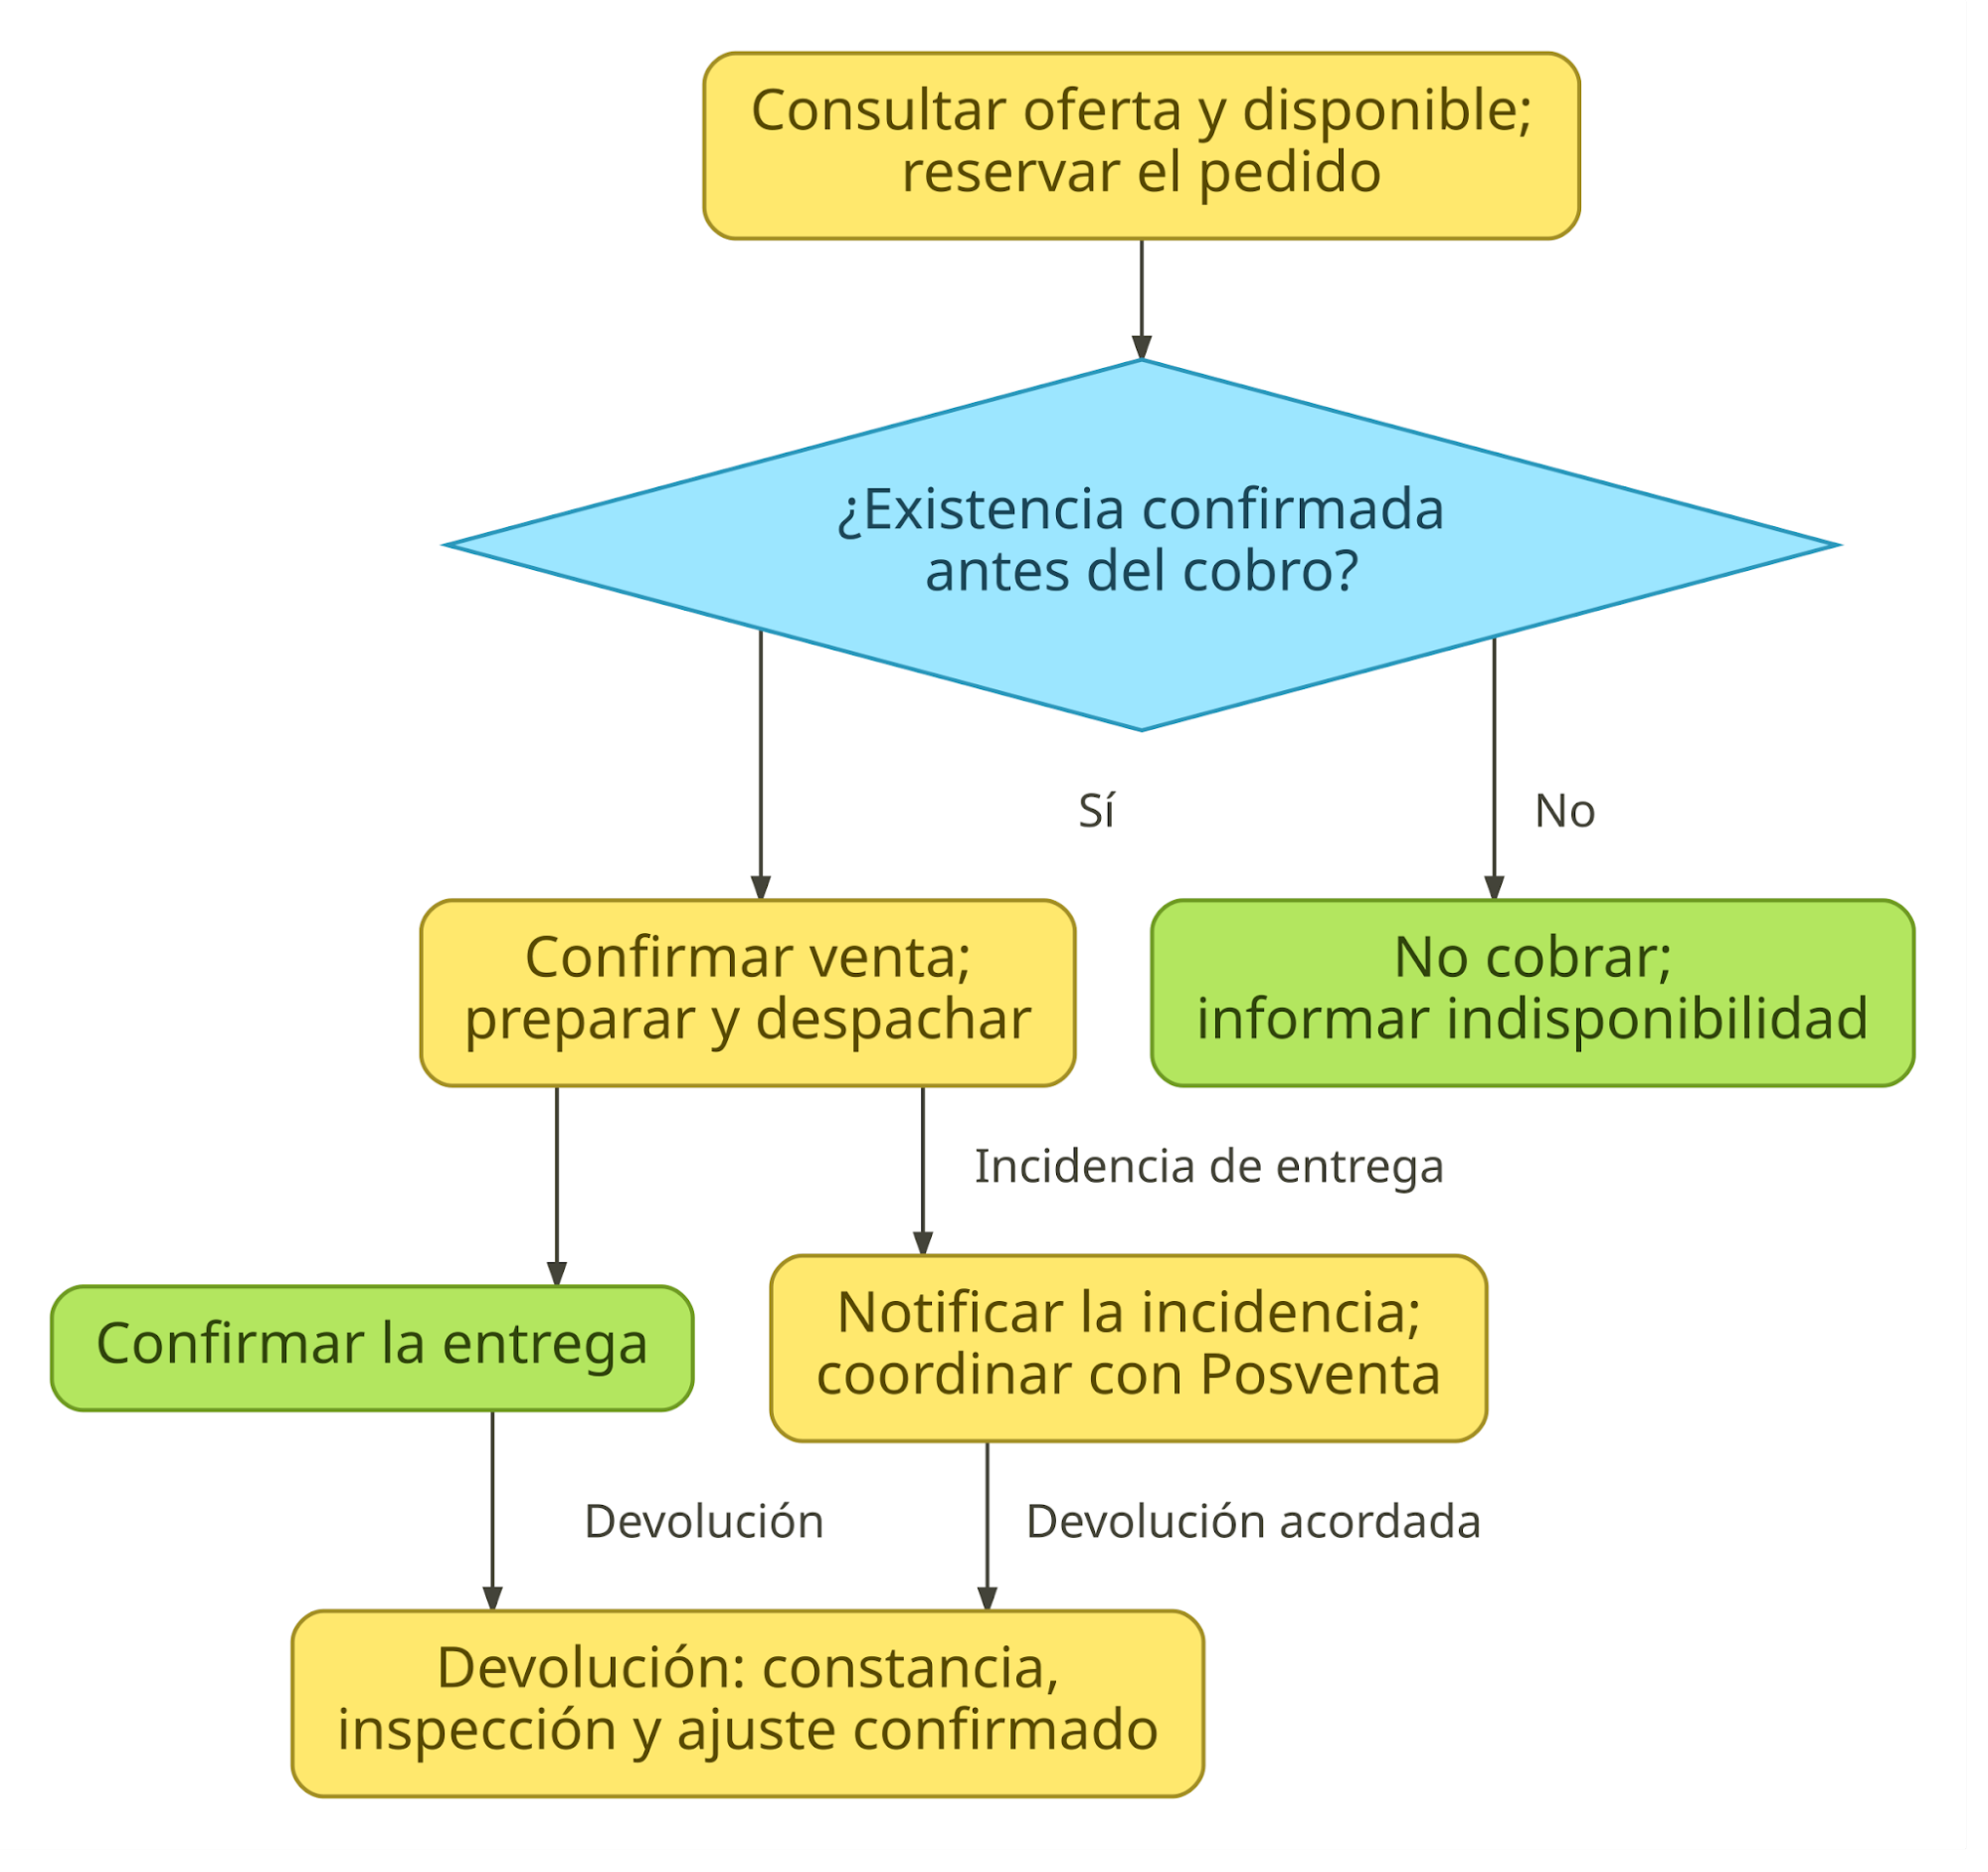
\includegraphics{figuras/sd-03_fig-3-6.png}}\end{center}

{Fuente: elaboración propia; diagrama editable en }{Miro}{.}

{El recorrido consulta la oferta y el disponible, reserva y confirma la existencia antes del cobro. Después registra la venta y coordina la preparación y entrega. Las ramas de excepción informan al cliente y derivan la incidencia a posventa; la devolución exige constancia, inspección y ajuste confirmado. Los rótulos abrevian los nombres del catálogo de 3.3.}

\subsection{3.4.4 La promesa de crédito}

{En el mostrador, la solicitud de tarjeta se tramita bajo el rol financiero. El Servicio de originación de crédito confirma la apertura solo cuando el Servicio de evidencia financiera acredita la entrega previa de información, su versión y aceptación, conforme a 3.3. La prueba comprobará el orden de esos actos y la recuperación del expediente, además de una evaluación en ocho segundos o menos (Caso 09, RT-09.01).}

{En una repactación, el Servicio de cartera de crédito consulta la evidencia antes de registrar las nuevas condiciones. Cada ola de migración se acepta cuando los saldos pueden conciliarse y el cobro continúa; una divergencia detiene el avance y activa el retorno ensayado.}

{La compra con tarjeta propia aplica el intercambio condicionado de 3.3. Su prueba deberá demostrar que Retail recibe únicamente el resultado transaccional autorizado y que una solicitud comercial ajena a esa finalidad se deniega y registra. Para aperturas y repactaciones, se comprobará el bloqueo ante evidencia insuficiente y la recuperación de los expedientes autorizados.}

{Las Figuras 3.7 y 3.8 presentan por separado la originación de crédito y la compra con tarjeta. La separación distingue la decisión financiera del control sobre los datos comunicados a Retail.}

{Figura 3.7. Originación de crédito dentro del ámbito del Emisor.}

\begin{center}\pandocbounded{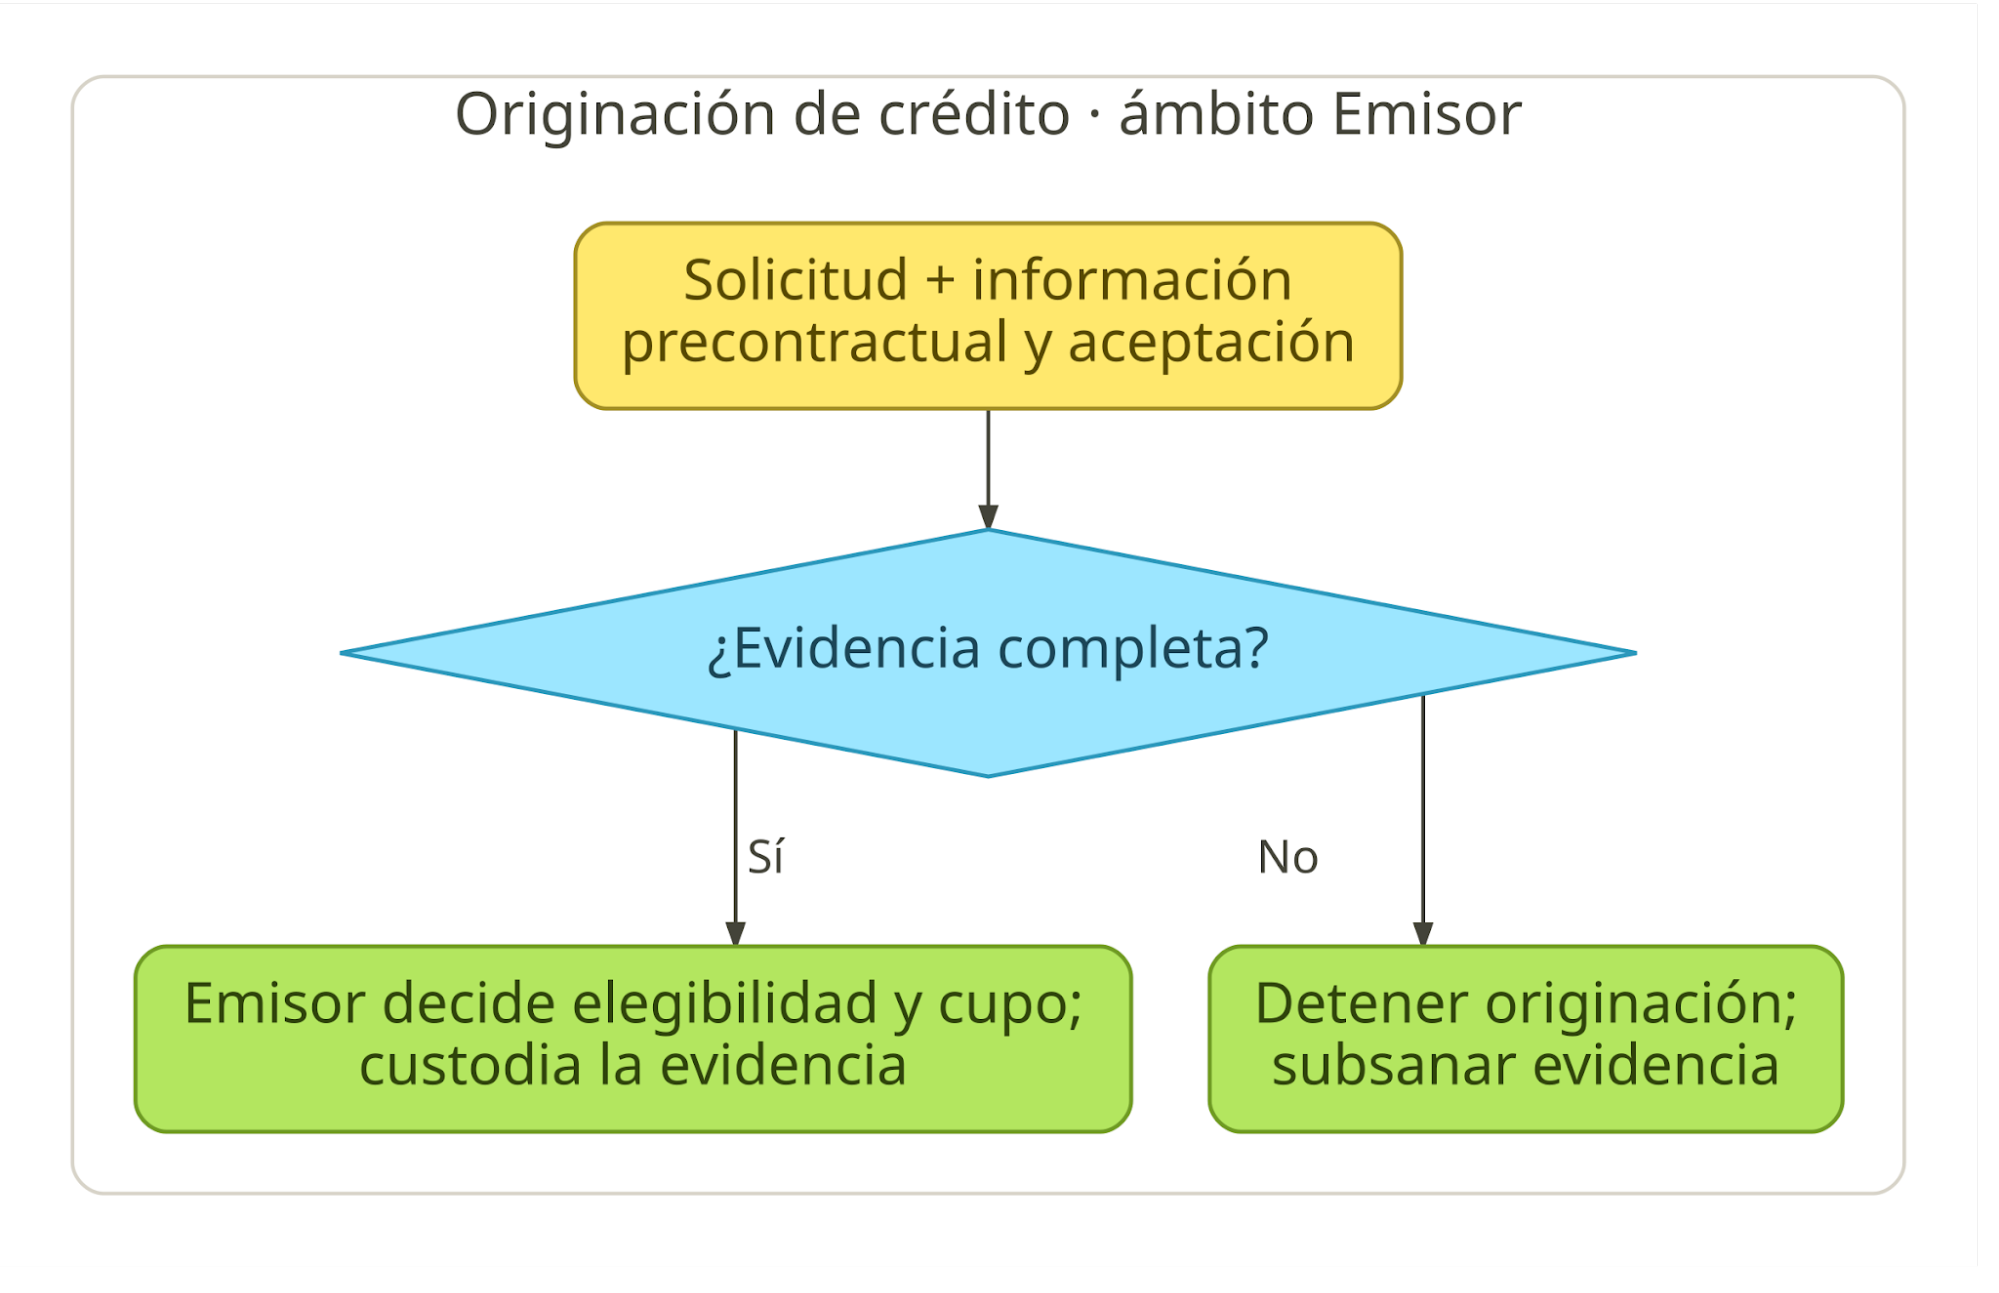
\includegraphics{figuras/sd-03_fig-3-7.png}}\end{center}

{Fuente: elaboración propia; diagrama editable en }{Miro}{.}

{La solicitud incorpora la información precontractual y su aceptación verificable. La evidencia completa permite al Emisor decidir la elegibilidad y el cupo; su ausencia detiene el trámite hasta subsanarla. Este recorrido conserva la decisión y el expediente en el ámbito financiero.}

{La Figura 3.8 muestra la autorización de una compra concreta y el control del intercambio necesario para responder a Retail.}

{Figura 3.8. Autorización de compra con tarjeta y respuesta limitada a Retail.}

\begin{center}\pandocbounded{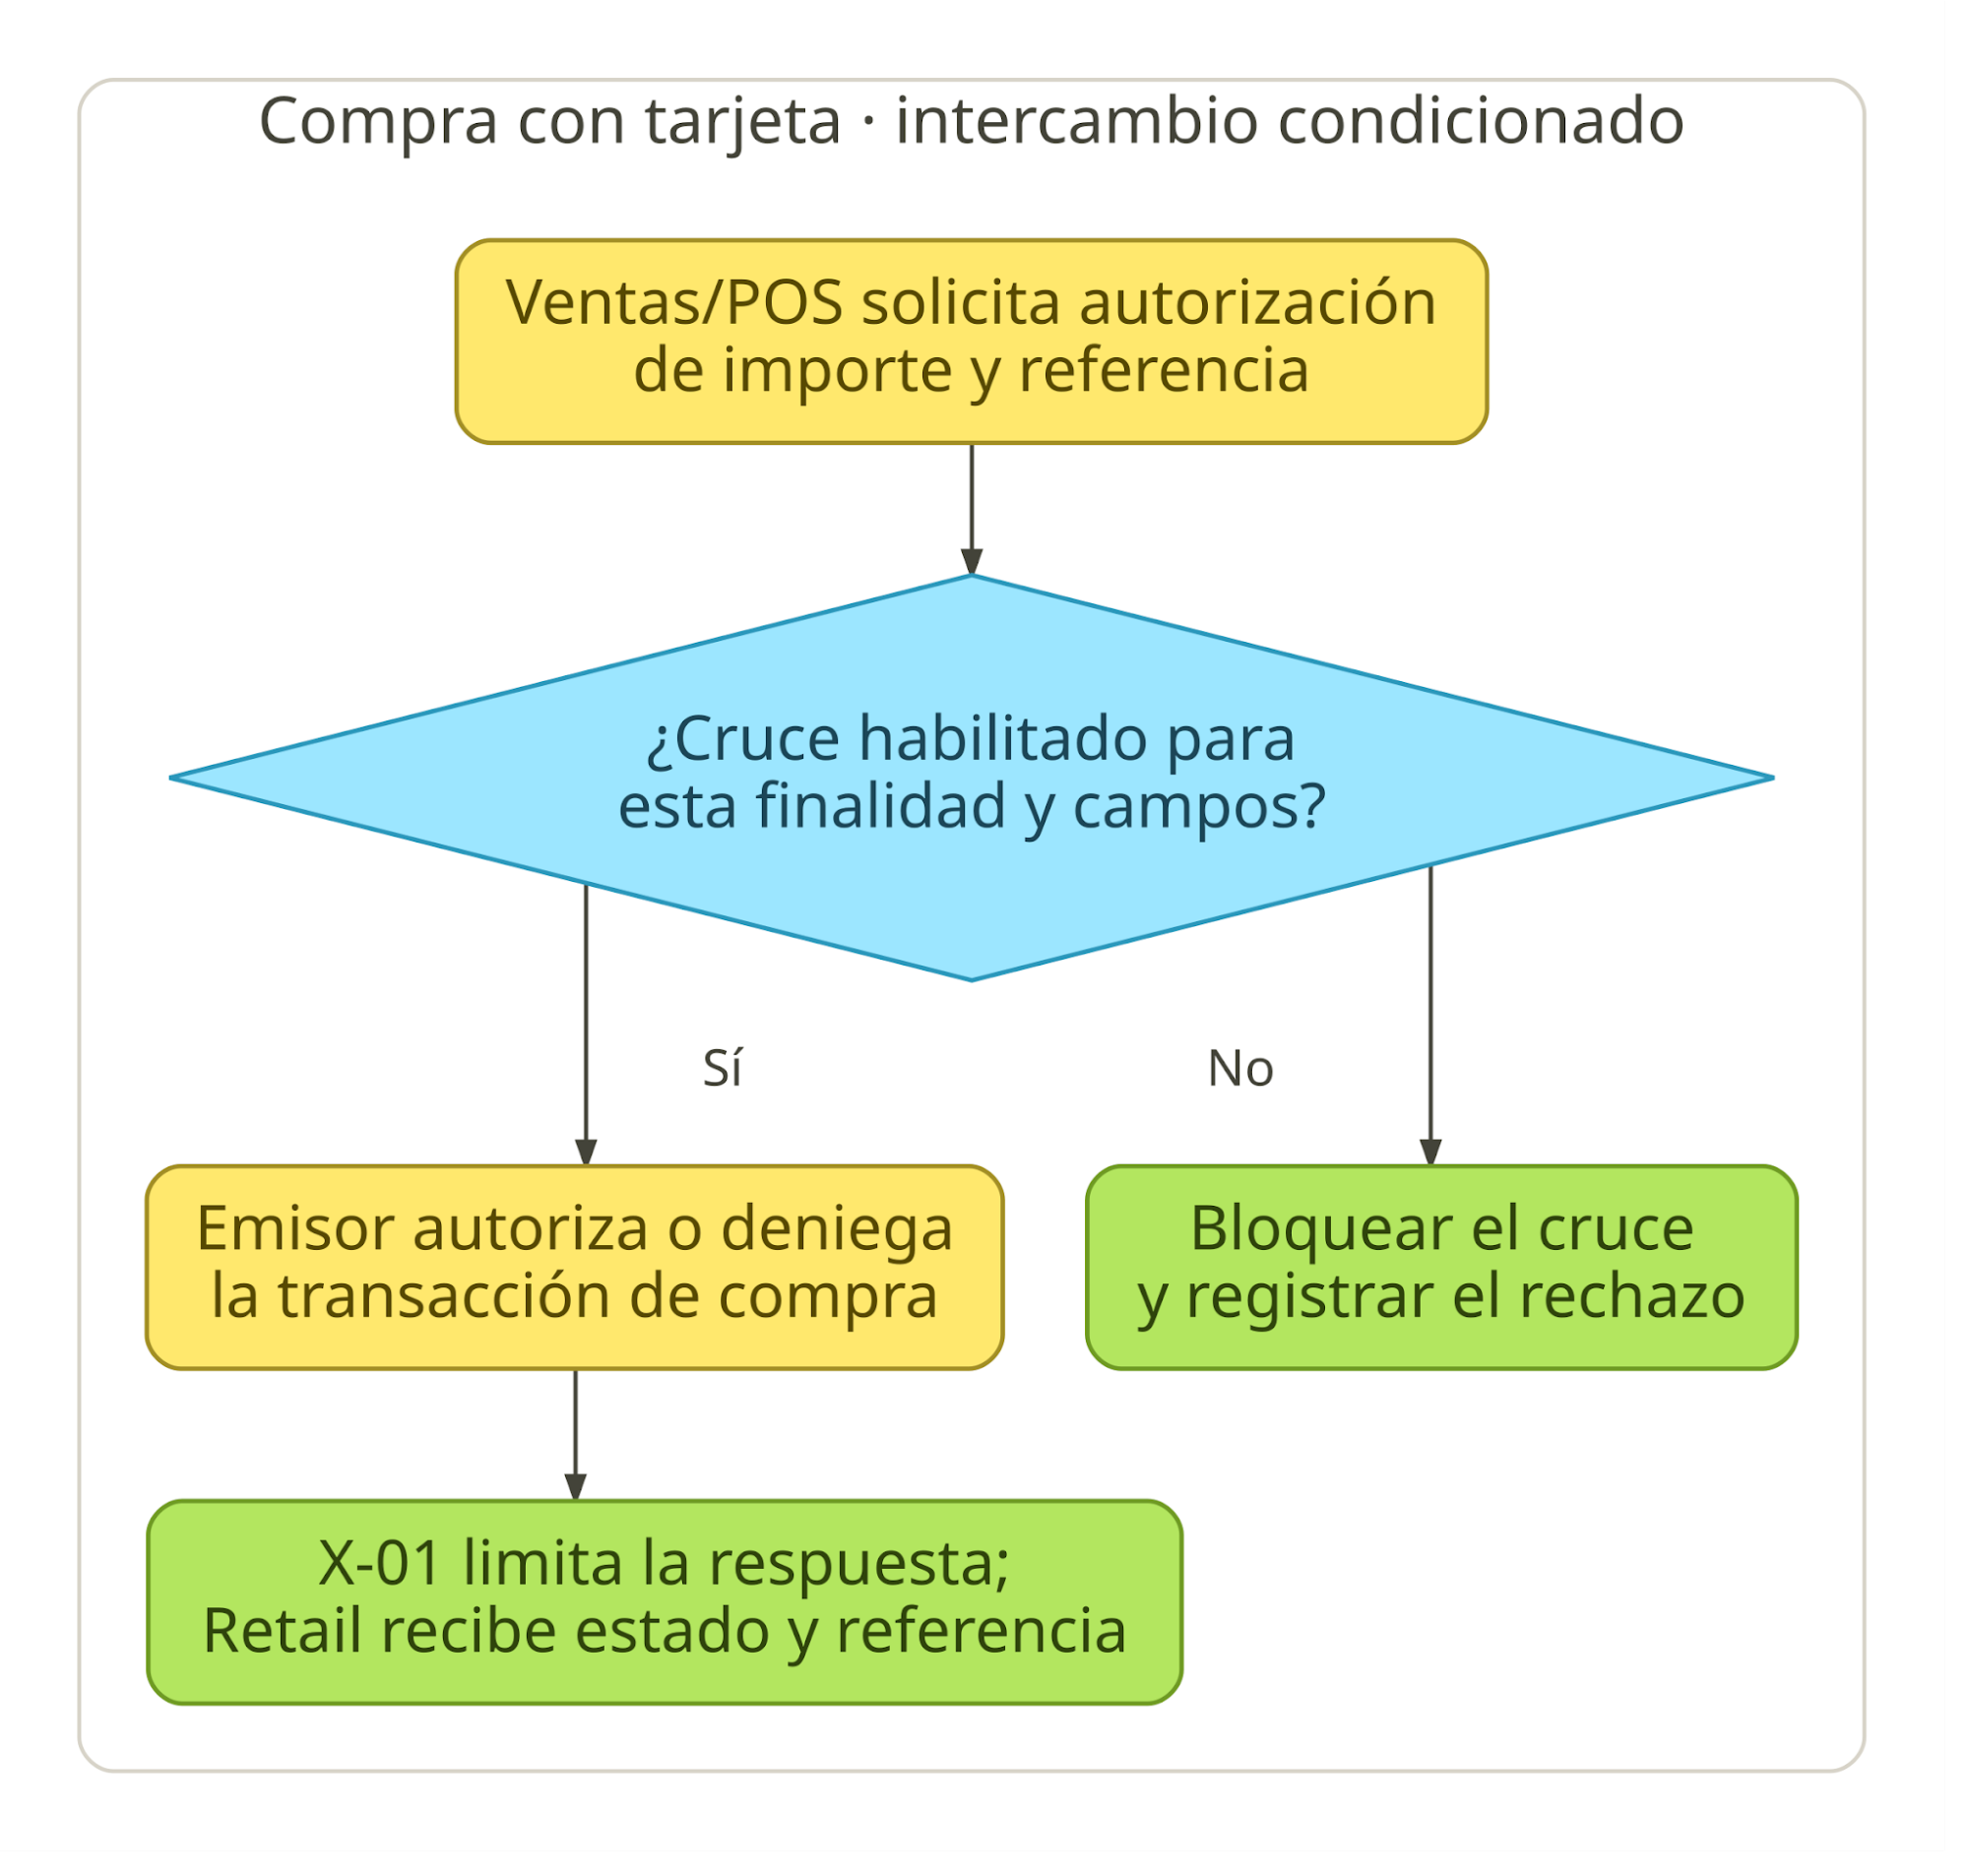
\includegraphics{figuras/sd-03_fig-3-8.png}}\end{center}

{Fuente: elaboración propia; diagrama editable en }{Miro}{.}

{Ventas/POS solicita una autorización por importe y referencia. Si el cruce está habilitado para esa finalidad y sus campos, el Emisor autoriza o deniega la transacción y X-01 limita el resultado comunicado; de otro modo, bloquea el cruce y registra el rechazo. La aceptación de crédito no habilita por sí sola el intercambio ni autoriza una compra posterior.}

\subsection{3.4.5 Continuidad y transición}

{Las promesas deben sostenerse durante pérdidas de enlace y durante el reemplazo gradual de plataformas. Durante la desconexión, la tienda completa venta, cobro, aplicación de promociones vigentes y consulta de existencia local; al volver el enlace, el Servicio de ventas concilia los hechos para evitar duplicidades o pérdida. La emisión tributaria sigue bajo autoridad de ERP/DTE y requiere una modalidad de contingencia aprobada y probada antes de comprometer la operación sin enlace. En ese estado no se originan tarjetas nuevas ni se amplían cupos. La modalidad de compra con crédito durante la desconexión requiere decisión de riesgo, pruebas y ruta de contingencia conforme al Caso 09, apartado 16.1. La continuidad local se compromete por 24 horas y se verifica con un corte de esa duración y retorno ensayado en el piloto (Bases Transversales, RT-03.10; 3.2).}

{La continuidad entre etapas se controla mediante convivencia, conciliación y retorno ensayado; sus compuertas e hitos se rigen por 3.2 y el artículo 17 de las Bases Administrativas. Cuando una falla impide recibir una decisión del Emisor, no se confirma una apertura ni una ampliación de cupo. Si falla un intercambio, su estado se conserva para verificar la conciliación antes de reanudar el flujo; la falta de respuesta no se interpreta como autorización. La prueba deberá demostrar ese comportamiento y la recuperación sin duplicar operaciones.}

\subsection{3.4.6 Apoyo de los actores}

{La estrategia aplica el análisis de influencia e interés de 2.4 mediante responsabilidades y resultados observables. La dirección y la Contraparte Técnica recibirán, antes de cada avance, los indicadores de las cuatro promesas, las incidencias y la evidencia de retorno. Su apoyo se buscará mediante decisiones de avance fundamentadas en esos resultados. TI coordinará con los responsables de cada servicio las pruebas de conciliación y recuperación, registrando operaciones sin conciliar, duplicidades y resultados del retorno.}

{Comercial y las jefaturas de tienda revisarán las campañas y el estado de exhibición; comprobarán el tiempo de propagación, las etiquetas confirmadas y las diferencias detectadas por muestreo. Logística e inventario coordinarán conteos y pruebas de reserva; medirán diferencias por categoría y nodo y cancelaciones por falta de existencia. Canales digitales contrastará lo publicado con la reserva y la entrega, utilizando los mismos registros que sostienen esas promesas.}

{Las jefaturas de tienda y el área responsable de capacitación organizarán ejercicios breves y repetibles para vendedores, cajeros y personal temporal, considerando la rotación anual del 62 \% y los aproximadamente 1.100 repositores externos (Caso 09, RT-12.11). La habilitación se comprobará mediante tareas ejecutadas correctamente por rol; los terceros accederán solo a las funciones que les correspondan. Vendedores y responsables de remuneraciones revisarán pedidos entre canales para comprobar la atribución de comisiones y registrar discrepancias que puedan desincentivar la preparación desde tienda.}

{La sustitución del POS se acompañará de pruebas de tareas con cajeros nuevos y experimentados. El prototipo cubrirá la venta ordinaria y la resolución de precio divergente, existencia incierta y venta sin enlace, además del paso autorizado hacia el rol financiero. Los participantes deberán reconocer el estado de cada operación y la acción siguiente sin confundir los datos comerciales con los financieros. Se registrarán tiempo de resolución, errores, intervenciones de supervisión y tiempo de aprendizaje por perfil; el diseño se ajustará con esos resultados antes del despliegue.}

{Atención y posventa coordinarán ejercicios de devolución y garantía; comprobarán constancias entregadas, destino físico de la unidad y avisos a vendedores externos. Los responsables de marketplace y logística acordarán con vendedores y transportistas los estados y avisos exigibles, y medirán su entrega y cumplimiento. El Emisor y la unidad de Contraloría y Cumplimiento evaluarán la integridad de los expedientes y el bloqueo de pasos incompletos. Clientes y titulares participarán en pruebas de comprensión de precios, entrega e información crediticia, verificando que puedan explicar las condiciones recibidas. Estas responsabilidades se proponen para la implantación y sus resultados deberán registrarse antes de afirmar que la adopción fue alcanzada.}

{Antes de aprobar este recorrido se completarán la memoria de capacidad y esfuerzo del disponible y la calibración de su margen; se definirán la resolución de diferencias de stock posteriores a la promesa, la política ante diferencias entre etiqueta y caja, y la alternativa de continuidad si falla la prueba de la plataforma financiera de 2011. La revisión conjunta de esta sección y 4.1 validará los contratos y responsables.}


\section*{Referencias}
\addcontentsline{toc}{section}{Referencias}

Multitiendas Ancoa S.A. (2026a). \textit{Bases administrativas para la preparación de la propuesta} (Licitación N.° TFEP-01/2026, versión 1.0).

Multitiendas Ancoa S.A. (2026b). \textit{Bases técnicas. Caso 09: Cadena multitienda} (Licitación N.° TFEP-01/2026, versión 1.0).

Multitiendas Ancoa S.A. (2026c). \textit{Bases técnicas transversales} (Licitación N.° TFEP-01/2026, versión 1.0).

Project Management Institute. (2017). \textit{A guide to the project management body of knowledge (PMBOK guide)} (6.ª ed.). Project Management Institute.

\section*{Declaración de uso de IA}
\addcontentsline{toc}{section}{Declaración de uso de IA}

Las secciones 3.1 y 3.2 se redactaron con asistencia de un modelo de lenguaje (Claude, de Anthropic) a partir de las decisiones de alcance tomadas por el equipo de Only Simple Solutions y de sus documentos de trabajo. El equipo definió los objetivos, las exclusiones, los supuestos y el reparto entre etapas. El modelo propuso la redacción y contrastó las cifras con las Bases. La sección 3.1 se revisó además con la herramienta humanizer, restringida a eliminar patrones de escritura automática sin alterar cifras, nombres ni citas, y con un lector automatizado que simuló a un interesado sin formación informática. Un integrante del equipo aprobó cada párrafo de la sección 3.1 antes de incorporarlo. La revisión humana del texto se registra en el Formulario A-6.

\ossFinalPage

\end{document}
